\documentclass{beamer}
\usepackage{tikz,amsmath,hyperref,graphicx,stackrel,animate}
\usetikzlibrary{positioning,shadows,arrows,shapes,calc}
\DeclareMathOperator*{\argmax}{argmax}
\DeclareMathOperator*{\argmin}{argmin}
\DeclareMathOperator*{\softmax}{softmax}
\mode<presentation>{\usetheme{Frankfurt}}
\AtBeginSection[]
{
  \begin{frame}<beamer>
    \frametitle{Outline}
    \tableofcontents[currentsection,currentsubsection]
  \end{frame}
}
\title{Lecture 17: Neural Nets}
\author{Mark Hasegawa-Johnson\\These slides are in the public domain.}
\date{ECE 417: Multimedia Signal Processing, Fall 2023}  
\begin{document}

% Title
\begin{frame}
  \maketitle
\end{frame}

% Title
\begin{frame}
  \tableofcontents
\end{frame}


%%%%%%%%%%%%%%%%%%%%%%%%%%%%%%%%%%%%%%%%%%%%
\section{Intro}
\setcounter{subsection}{1}
\begin{frame}
  \frametitle{What is a Neural Network?}
  \begin{itemize}
  \item Computation in biological neural networks is performed by
    billions of simple cells (neurons), each of which performs one
    very simple computation.
  \item Biological neural networks learn by strengthening  the connections
    between some pairs of neurons, and weakening other connections.
  \end{itemize}
\end{frame}

\begin{frame}
  \frametitle{What is an Artificial Neural Network?}
  \begin{itemize}
  \item Computation in an artificial neural network is performed by
    millions of simple cells (nodes), each of which performs one
    very simple computation.
  \item Artificial neural networks learn by strengthening  the connections
    between some pairs of nodes, and weakening other connections.
  \end{itemize}
\end{frame}

\begin{frame}
  \frametitle{Two-Layer Feedforward Neural Network}
  \begin{small}\begin{center}
  \tikzstyle{pre}=[<-,shorten <=1pt,>=stealth',semithick,draw=blue]
  \tikzstyle{post}=[->,shorten >=1pt,>=stealth',semithick,draw=blue]
  \begin{tikzpicture}[
      open/.style={circle,thick, draw=blue, text=black, align=left, text width=0.5cm}
    ]
    \node (x0) at (0,0.25) {$1$};
    \node[open] (x1) at (1,0) {$x_1$};
    \node[open] (x2) at (2,0) {$x_2$};
    \node (x3) at (2.75,0) {\ldots};
    \node[open] (xm0) at (3.5,0) {$x_{m_0}$};
    \node (input) at (6,0) {$\mathbf{a}_0=\mathbf{x}$ is the input vector};
    \node[open] (z11) at (1,1.3) {$z_{1,1}$} edge[pre](x0) edge[pre](x1) edge[pre](x2) edge[pre](xm0);
    \node[open] (z12) at (2,1.3) {$z_{1,2}$} edge[pre](x0) edge[pre](x1) edge[pre](x2) edge[pre](xm0);
    \node (z13) at (2.75,1.3) {\ldots};
    \node[open] (z1m1) at (3.5,1.3) {$z_{1,m_1}$} edge[pre](x0) edge[pre](x1) edge[pre](x2) edge[pre](xm0);
    \node (z1eq) at (6,1.3) {$\mathbf{z}_1=\mathbf{W}_1\mathbf{x}+\mathbf{b}_1$};
    \node (a10) at (0,2.7) {$1$};
    \node[open] (a11) at (1,2.45) {$a_{1,1}$} edge[pre](z11);
    \node[open] (a12) at (2,2.45) {$a_{1,2}$} edge[pre](z12);
    \node (a13) at (2.75,2.45) {\ldots};
    \node[open] (a1m1) at (3.5,2.45) {$a_{1,m_1}$} edge[pre](z1m1);
    \node (a1eq) at (6,2.45) {$\mathbf{a}_1=\mathbf{f}_1(\mathbf{z}_1)$};
    \node[open] (z21) at (1,3.75) {$z_{2,1}$} edge[pre](a10) edge[pre](a11) edge[pre](a12) edge[pre](a1m1);
    \node[open] (z22) at (2,3.75) {$z_{2,2}$} edge[pre](a10) edge[pre](a11) edge[pre](a12) edge[pre](a1m1);
    \node (z23) at (2.75,3.75) {\ldots};
    \node[open] (z2m2) at (3.5,3.75){$z_{2,m_2}$}edge[pre](a10) edge[pre](a11) edge[pre](a12) edge[pre](a1m1);
    \node (z2eq) at (6,3.75) {$\mathbf{z}_2=\mathbf{W}_2\mathbf{a}_1+\mathbf{b}_2$};
    \node[open] (a21) at (1,4.9) {$g_{1}$} edge[pre](z21);
    \node[open] (a22) at (2,4.9) {$g_{2}$} edge[pre](z22);
    \node (a23) at (2.75,4.9) {\ldots};
    \node[open] (a2m2) at (3.5,4.9) {$g_{m_2}$} edge[pre](z2m2);
    \node (z2eq) at (6,4.9) {$\mathbf{g}(\mathbf{x})=\mathbf{a}_2=\mathbf{f}_2(\mathbf{z}_2)$};
    \node (output) at (2.2,5.65) {${\mathcal{L}}=E\left[-\ln\Pr(\mathbf{y}|\mathbf{g}(\mathbf{x}))\right]$};
  \end{tikzpicture}
\end{center}
\end{small}
\end{frame}

\begin{frame}
  \frametitle{Why use neural nets?}

  Barron (1993) showed that a neural net is a {\bf universal
    approximator:} it can approximate any function arbitrarily well,
  if the number of hidden nodes is large enough.  Assume:
  \begin{itemize}
  \item Linear output nodes: $\mathbf{g}(\mathbf{x})=\mathbf{a}_2=\mathbf{z}_2$
  \item Hidden nodes are $n$ smooth scalar nonlinearities:
    \begin{displaymath}
      a_{1,k}=f_1(z_{1,k}),~~1\le k\le m_1,~\mbox{where}~
      \frac{\partial a_{1,k}}{\partial z_{1,k}}~\text{is finite}
    \end{displaymath}
  \item Smooth target function: The target vectors $\mathbf{y}$ are
    all computed by some function $\mathbf{y}(\mathbf{x})$ that is
    unknown but smooth (its Fourier transform has finite first moment)
  \end{itemize}
  \begin{displaymath}\text{Then:}~~~~
  \max_{\mathbf{y}(\mathbf{x})}
  \min_{\mathbf{g}(\mathbf{x})}
  E\left[\Vert\mathbf{y}(\mathbf{x})-\mathbf{g}(\mathbf{x})\Vert^2\right]
  \le {\mathcal O}\left\{\frac{1}{m_1}\right\}
  \end{displaymath}
\end{frame}

%%%%%%%%%%%%%%%%%%%%%%%%%%%%%%%%%%%%%%%%%%%%%%%%%%%%%%%%%%%%%%%
\section[Classification]{Classification Example: Arbitrary Classifier}
\setcounter{subsection}{1}

\begin{frame}
  \frametitle{Target: Can we get the neural net to compute this
    function?}

  Suppose our goal is to find some weights and biases, $\mathbf{W}_1$,
  $\mathbf{b}_1$, $\mathbf{W}_2$, and $\mathbf{b}_2$ so that the
  output activation is a scalar binary classifier that classifies
  every pixel $\mathbf{x}=[x_1,x_2]$ as being either ``red'' or
  ``blue,'' where the ground truth is shown in this picture:

  \centerline{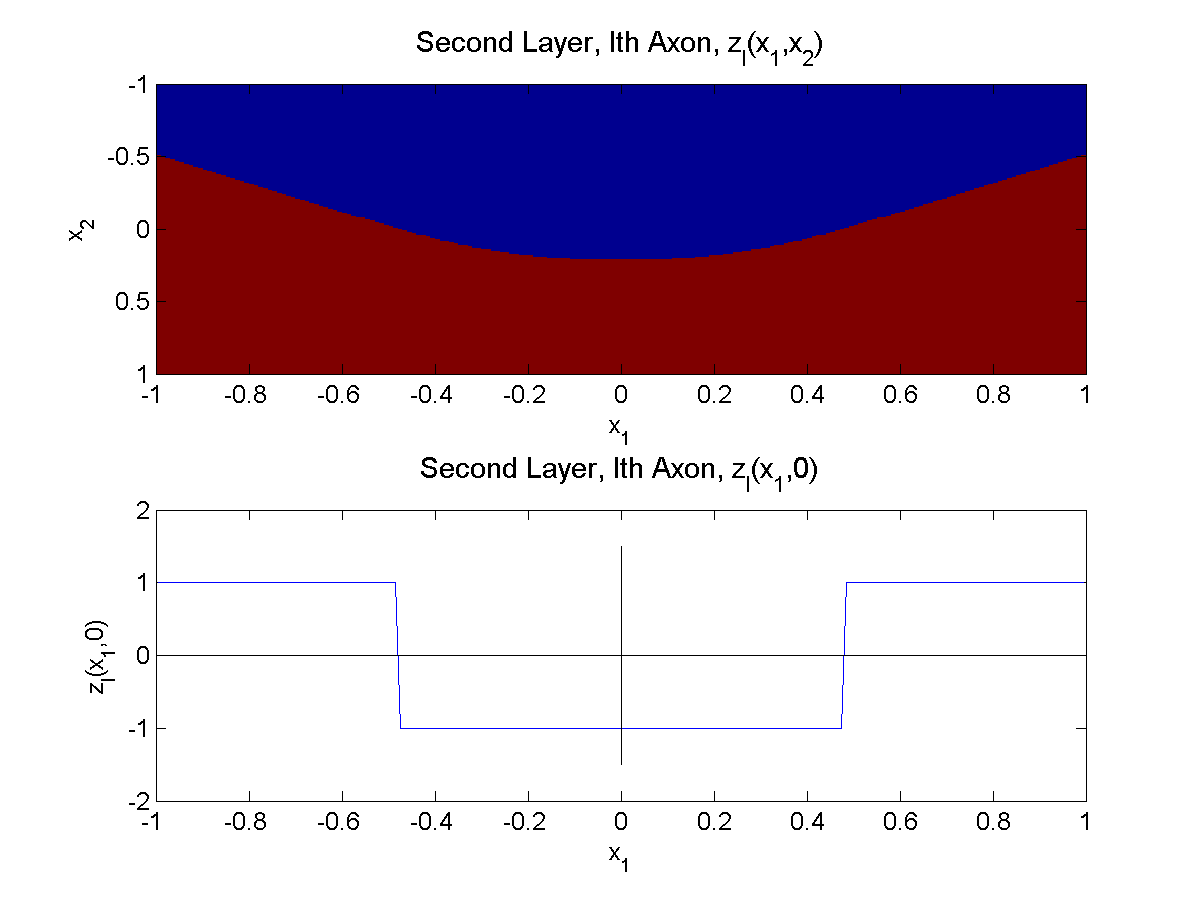
\includegraphics[width=3in]{figs/nn_axon2.png}}
\end{frame}

\begin{frame}
  \frametitle{First Layer Excitation:
    $\mathbf{z}_{1}=\mathbf{b}_{1}+\mathbf{W}_1\mathbf{x}$} The first
  layer of the neural net just computes a linear function of
  $\mathbf{x}$. Here's an example:
  \centerline{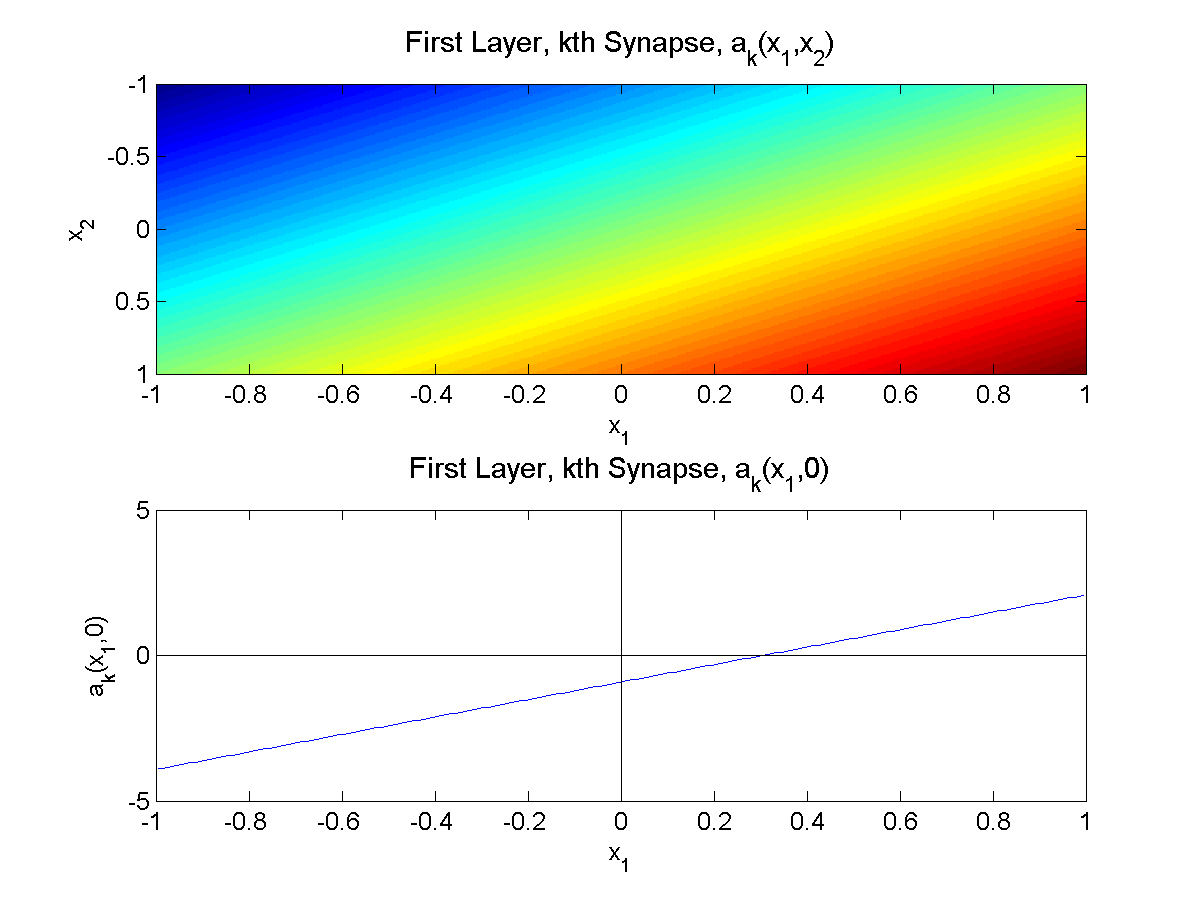
\includegraphics[width=3in]{figs/nn_synapse1.png}}
\end{frame}

\begin{frame}
  \frametitle{First Layer Activation: $\mathbf{a}_{1}=\tanh(\mathbf{z}_{1})$}

  The activation nonlinearity then ``squashes'' the linear function:
  \centerline{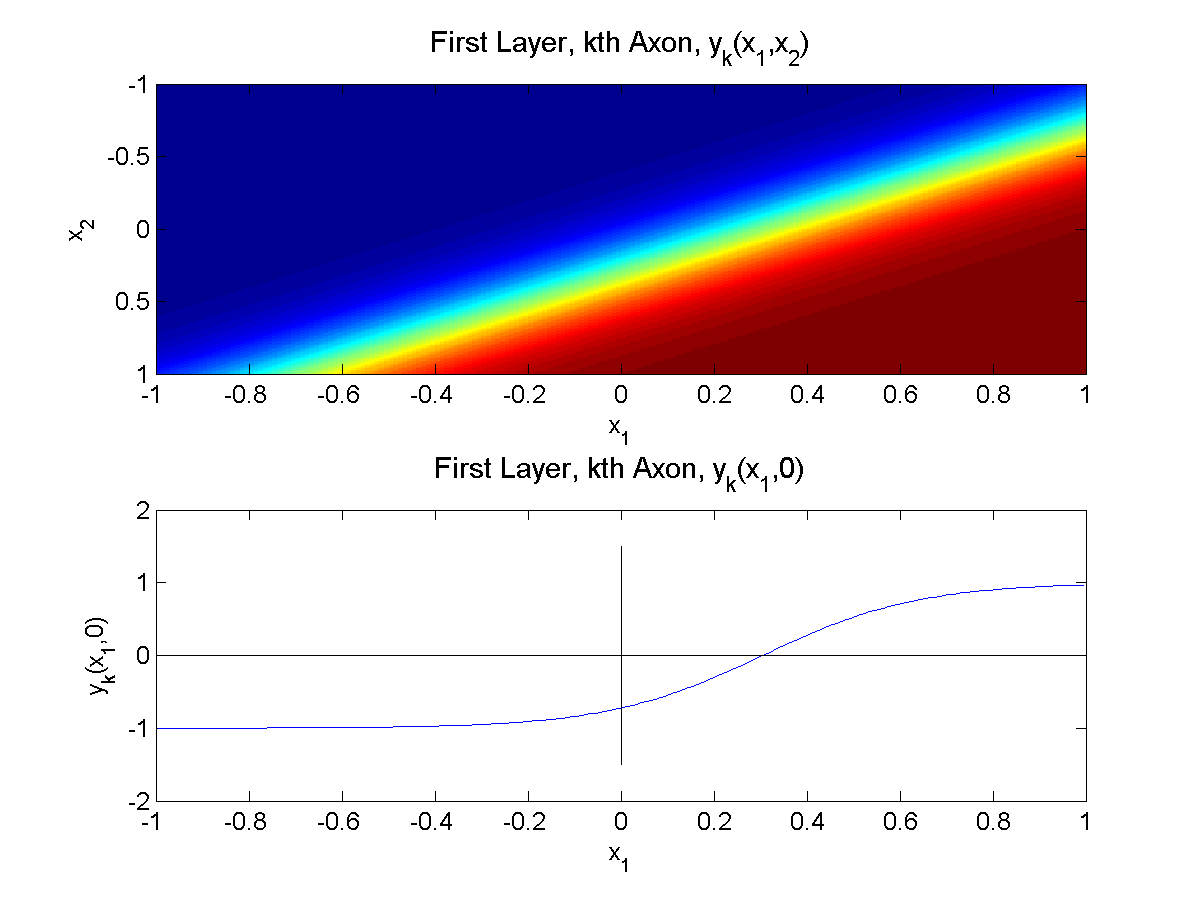
\includegraphics[width=3in]{figs/nn_axon1.png}}
\end{frame}

\begin{frame}
  \frametitle{Second Layer Excitation:
    $z_{2}=b_{2}+\mathbf{w}_2^T\mathbf{a}_{1}$}

  The second layer then computes a linear combination of the
  first-layer activations:
  \centerline{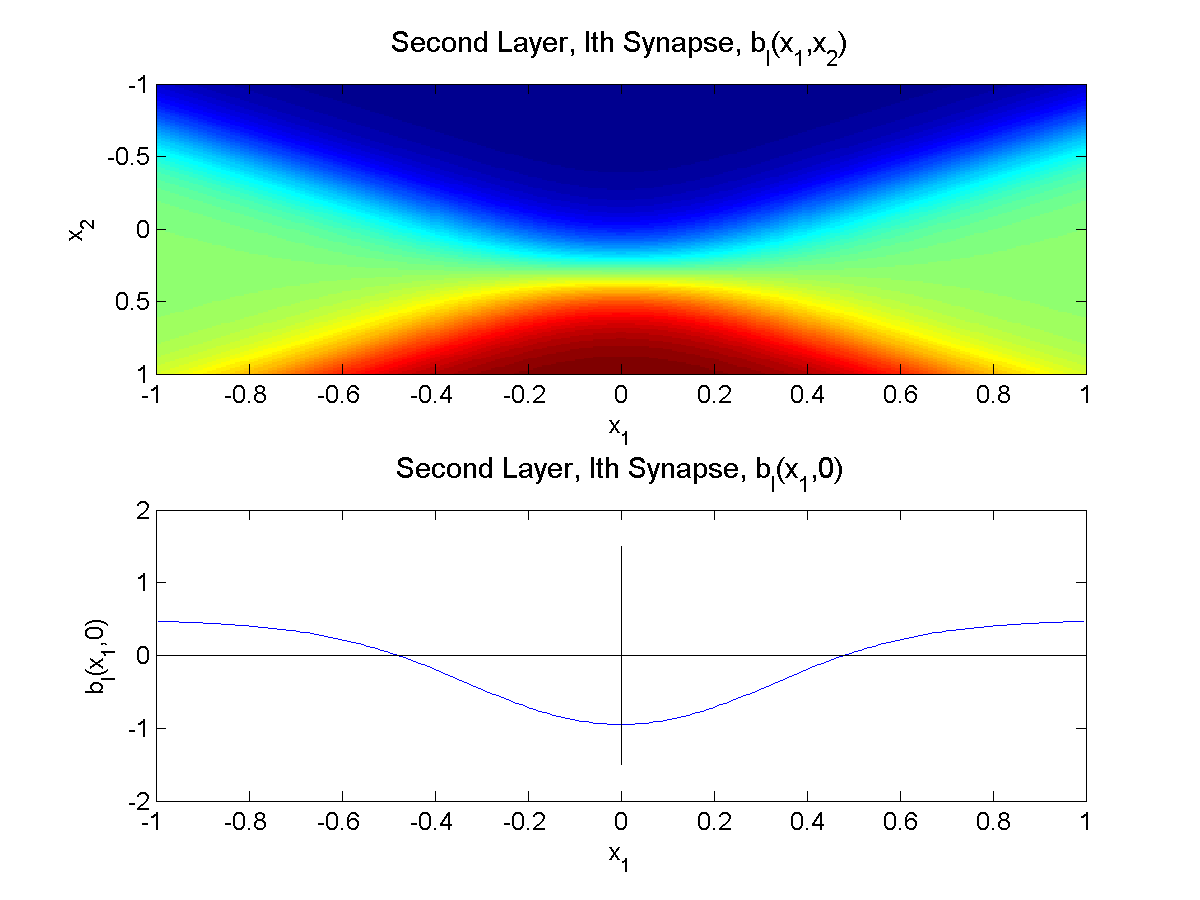
\includegraphics[width=3in]{figs/nn_synapse2.png}}
\end{frame}

\begin{frame}
  \frametitle{Second Layer Activation: $a_2=u(z_2)$}

  The second layer activation is then just a binary threshold, $a_2=1$
  if $z_2>0$, otherwise $a_2=0$:
  
  \centerline{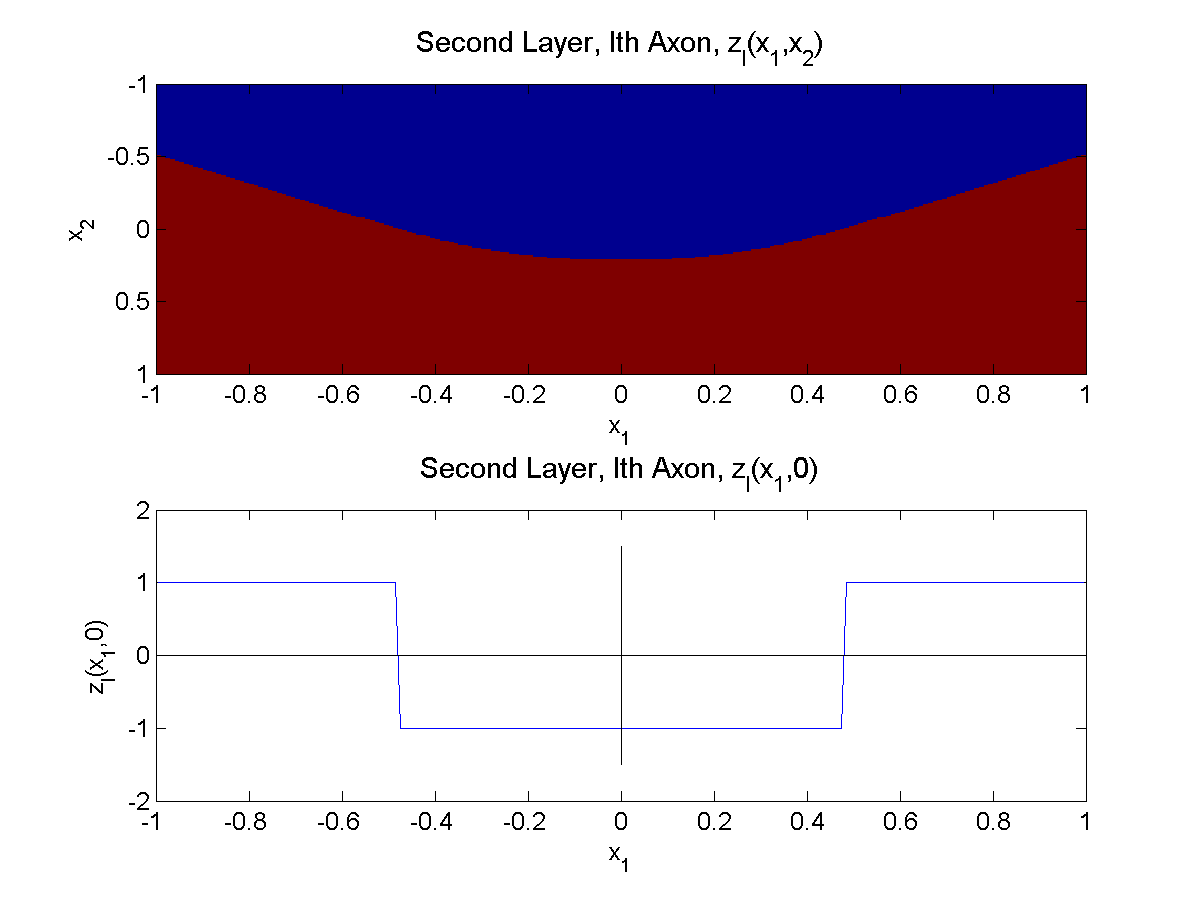
\includegraphics[width=3in]{figs/nn_axon2.png}}
\end{frame}


%%%%%%%%%%%%%%%%%%%%%%%%%%%%%%%%%%%%%%%%%%%%%%%%%%%%%%%%%%%%%%%
\section[Regression]{Regression Example: Semicircle $\rightarrow$ Parabola}
\setcounter{subsection}{1}

\begin{frame}
  \frametitle{Example \#2: Semicircle $\rightarrow$ Parabola}

  Can we design a neural net that converts a semicircle
  ($x_1^2+x_2^2=1$) to a parabola ($y_2=y_1^2$)?
  \centerline{\includegraphics[height=2in]{exp/nn_target_figure.png}}
\end{frame}

\begin{frame}
  \frametitle{Two-Layer Feedforward Neural Network}
  \begin{small}\begin{center}
  \tikzstyle{pre}=[<-,shorten <=1pt,>=stealth',semithick,draw=blue]
  \tikzstyle{post}=[->,shorten >=1pt,>=stealth',semithick,draw=blue]
  \begin{tikzpicture}[
      open/.style={circle,thick, draw=blue, text=black, align=left, text width=0.5cm}
    ]
    \node (x0) at (0,0.25) {$1$};
    \node[open] (x1) at (1,0) {$x_1$};
    \node[open] (x2) at (2,0) {$x_2$};
    \node (x3) at (2.75,0) {\ldots};
    \node[open] (xm0) at (3.5,0) {$x_{m_0}$};
    \node (input) at (6,0) {$\mathbf{a}_0=\mathbf{x}$ is the input vector};
    \node[open] (z11) at (1,1.3) {$z_{1,1}$} edge[pre](x0) edge[pre](x1) edge[pre](x2) edge[pre](xm0);
    \node[open] (z12) at (2,1.3) {$z_{1,2}$} edge[pre](x0) edge[pre](x1) edge[pre](x2) edge[pre](xm0);
    \node (z13) at (2.75,1.3) {\ldots};
    \node[open] (z1m1) at (3.5,1.3) {$z_{1,m_1}$} edge[pre](x0) edge[pre](x1) edge[pre](x2) edge[pre](xm0);
    \node (z1eq) at (6,1.3) {$\mathbf{z}_1=\mathbf{W}_1\mathbf{x}+\mathbf{b}_1$};
    \node (a10) at (0,2.7) {$1$};
    \node[open] (a11) at (1,2.45) {$a_{1,1}$} edge[pre](z11);
    \node[open] (a12) at (2,2.45) {$a_{1,2}$} edge[pre](z12);
    \node (a13) at (2.75,2.45) {\ldots};
    \node[open] (a1m1) at (3.5,2.45) {$a_{1,m_1}$} edge[pre](z1m1);
    \node (a1eq) at (6,2.45) {$\mathbf{a}_1=\mathbf{f}_1(\mathbf{z}_1)$};
    \node[open] (z21) at (1,3.75) {$z_{2,1}$} edge[pre](a10) edge[pre](a11) edge[pre](a12) edge[pre](a1m1);
    \node[open] (z22) at (2,3.75) {$z_{2,2}$} edge[pre](a10) edge[pre](a11) edge[pre](a12) edge[pre](a1m1);
    \node (z23) at (2.75,3.75) {\ldots};
    \node[open] (z2m2) at (3.5,3.75){$z_{2,m_2}$}edge[pre](a10) edge[pre](a11) edge[pre](a12) edge[pre](a1m1);
    \node (z2eq) at (6,3.75) {$\mathbf{z}_2=\mathbf{W}_2\mathbf{a}_1+\mathbf{b}_2$};
    \node[open] (a21) at (1,4.9) {$g_{1}$} edge[pre](z21);
    \node[open] (a22) at (2,4.9) {$g_{2}$} edge[pre](z22);
    \node (a23) at (2.75,4.9) {\ldots};
    \node[open] (a2m2) at (3.5,4.9) {$g_{m_2}$} edge[pre](z2m2);
    \node (z2eq) at (6,4.9) {$\mathbf{g}(\mathbf{x})=\mathbf{a}_2=\mathbf{f}_2(\mathbf{z}_2)$};
    \node (output) at (2.2,5.65) {${\mathcal{L}}=E\left[-\ln\Pr(\mathbf{y}|\mathbf{g}(\mathbf{x}))\right]$};
  \end{tikzpicture}
\end{center}
\end{small}
\end{frame}

\begin{frame}
  \frametitle{Example \#2: Semicircle $\rightarrow$ Parabola}

  Let's define some notation:
  \begin{itemize}
  \item {\bf Second Layer:} Define
    $\mathbf{w}_{2,:,j}=\left[\begin{array}{c}w_{2,1,j}\\w_{2,n,j}\end{array}\right]$,
    the $j^{\textrm{th}}$ column of the $\mathbf{W}_2$ matrix, so that
    \[
    \mathbf{W}_2=\left[\mathbf{w}_{2,:,1},\mathbf{w}_{2,:,2}\right]
    \]
  \item {\bf First Layer Excitation:} Define
    $\mathbf{w}_{1,k,:}^T=[w_{1,k,1},\ldots,w_{1,k,m}]$, the
    $k^{\textrm{th}}$ row of the $\mathbf{W}_1$ matrix, so that
    \[
    \mathbf{W}_1=\left[\begin{array}{c}\mathbf{w}_{1,1,:}^T\\\mathbf{w}_{1,2,:}^T\end{array}\right]
    \]
  \end{itemize}
\end{frame}

\begin{frame}
  \frametitle{Piece-Wise Constant Approximation}

  Suppose we want the NN to calculate a piece-wise constant approximation: 
  The second layer of the network approximates $\mathbf{y}$ using a bias term $\mathbf{b}_2$,
  plus correction vectors $\mathbf{w}_{2,:,j}$, each scaled by its activation $a_{1,j}$:
  \[
  \mathbf{g}(\mathbf{x}) = \mathbf{b}_2 + \sum_j \mathbf{w}_{2,:,j} a_{1,j}
  \]
  The first layer of the network decides whether or not to ``turn on'' each of the
  $a_{1,j}$'s.  It does this by comparing $\mathbf{x}$ to a series of linear threshold vectors:
  \[
  a_{1,j} = \sigma\left(\mathbf{w}_{1,k,:}^T\mathbf{x}\right)\approx\begin{cases}
  1 & \mathbf{w}_{1,k,:}^T\mathbf{x} > 0\\
  0 & \mathbf{w}_{1,k,:}^T\mathbf{x} < 0
  \end{cases}
  \]
\end{frame}

\begin{frame}
  \frametitle{Example \#2: Semicircle $\rightarrow$ Parabola}

  \includegraphics[width=1.2\textwidth]{exp/nnapprox0.png}
\end{frame}

\begin{frame}
  \frametitle{Example \#2: Semicircle $\rightarrow$ Parabola}

  \includegraphics[width=1.2\textwidth]{exp/nnapprox1.png}
\end{frame}

\begin{frame}
  \frametitle{Example \#2: Semicircle $\rightarrow$ Parabola}

  \includegraphics[width=1.2\textwidth]{exp/nnapprox2.png}
\end{frame}

\begin{frame}
  \frametitle{Example \#2: Semicircle $\rightarrow$ Parabola}

  \includegraphics[width=1.2\textwidth]{exp/nnapprox3.png}
\end{frame}

\begin{frame}
  \frametitle{Example \#2: Semicircle $\rightarrow$ Parabola}

  \includegraphics[width=1.2\textwidth]{exp/nnapprox4.png}
\end{frame}

\begin{frame}
  \frametitle{Example \#2: Semicircle $\rightarrow$ Parabola}

  \includegraphics[width=1.2\textwidth]{exp/nnapprox5.png}
\end{frame}

\begin{frame}
  \frametitle{Example \#2: Semicircle $\rightarrow$ Parabola}

  \includegraphics[width=1.2\textwidth]{exp/nnapprox6.png}
\end{frame}

\begin{frame}
  \frametitle{Example \#2: Semicircle $\rightarrow$ Parabola}

  \includegraphics[width=1.2\textwidth]{exp/nnapprox7.png}
\end{frame}


\begin{frame}
  \frametitle{Example \#2: Semicircle $\rightarrow$ Parabola}

  \includegraphics[width=1.2\textwidth]{exp/nnapprox8.png}
\end{frame}


%%%%%%%%%%%%%%%%%%%%%%%%%%%%%%%%%%%%%%%%%%%%
\section[Nonlinearities]{Scalar Nonlinearities}
\setcounter{subsection}{1}

\begin{frame}
  \frametitle{Scalar Nonlinearities}

  \begin{itemize}
  \item A layer might have a vector nonlinearity,
    $\mathbf{a}_l=\mathbf{f}_l(\mathbf{z}_l)$, in which case every
    element of $\mathbf{a}_l$ depends on every element of
    $\mathbf{z}_l$.  These are used rarely, because they're rarely
    necessary, and computation is hard.  The only one of these we'll
    ever use is the softmax.
  \item Most NN nonlinearities are scalar,
    $\mathbf{a}_l=f_l(\mathbf{z}_l$), which means that
    \begin{displaymath}
      \left[\begin{array}{c}a_{l,1}\\\vdots\\a_{l,m_l}\end{array}\right]=
      \left[\begin{array}{c}f_l(z_{l,1})\\\vdots\\f_l(z_{l,m_l})\end{array}\right]
    \end{displaymath}
  \end{itemize}
\end{frame}

\begin{frame}
  \begin{columns}[t]
    \begin{column}{1.85in}
      \begin{block}{The Basic Scalar  Nonlinearity: Unit Step (a.k.a. Heaviside function)}
        \[
        u\left(z\right)=\begin{cases}
        1 & z > 0\\
        0 & z < 0
        \end{cases}
        \]
        \centerline{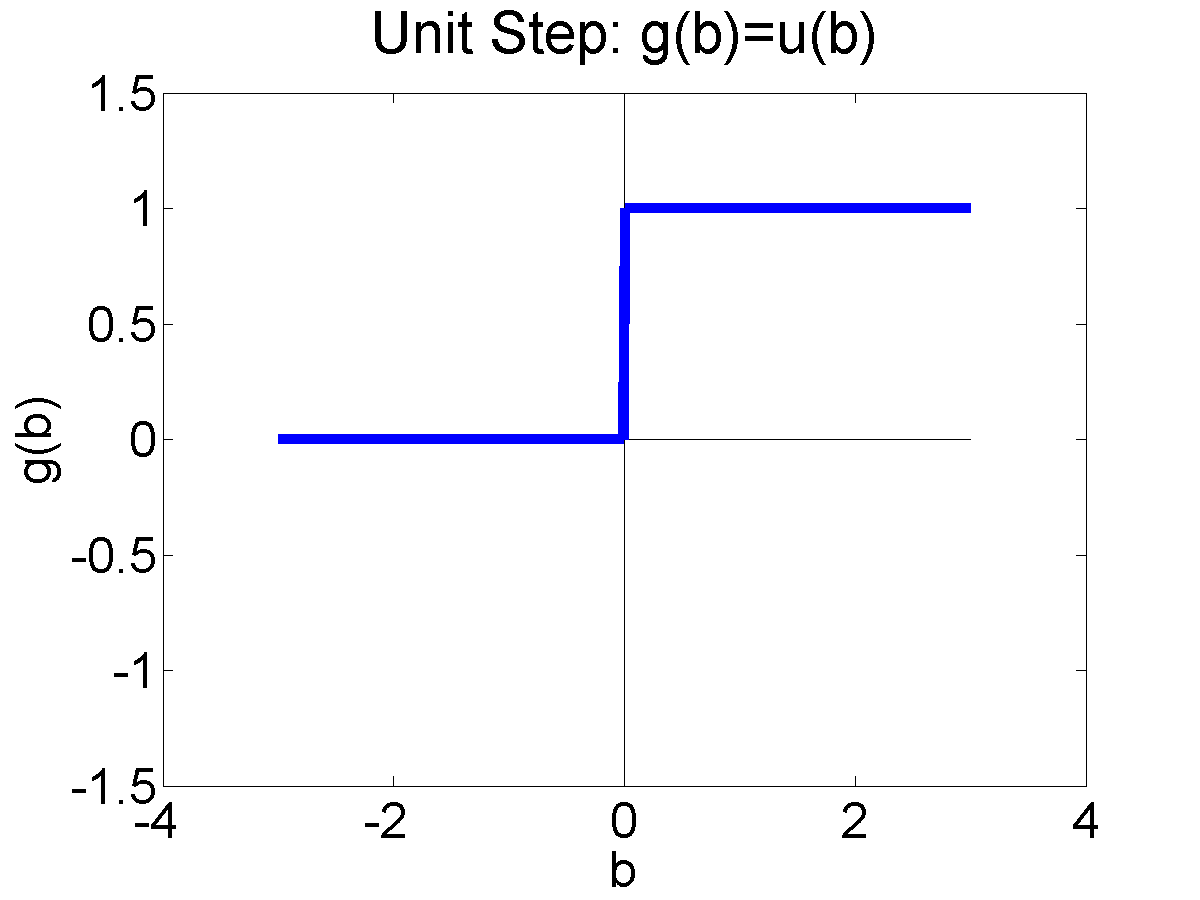
\includegraphics[width=1.75in]{figs/nn_unitstep.png}}
      \end{block}
    \end{column}
    \begin{column}{2.65in}
      \begin{block}{Pros and Cons of the Unit Step}
        \begin{itemize}
        \item {\bf Pro:} It gives exactly piece-wise constant
          approximation of any desired $y$.
        \item {\bf Con:} It's not differentiable, so we won't be able to
          use gradient descent to learn the network weights.
        \end{itemize}
        The derivative of the unit step is called the Dirac delta
        function, $\frac{\partial u}{\partial z}=\delta(z)$, where
        $\delta(z)$ is defined to be the function such that
        $\delta(0)=\infty$, $\delta(z)=0$ for any $z\ne 0$, and
        \begin{displaymath}
          \int_{-\epsilon}^\epsilon \delta(z)dz=1~\forall\epsilon\in\Re_{+}
        \end{displaymath}
      \end{block}
    \end{column}
  \end{columns}
\end{frame}

\begin{frame}
  \begin{columns}[t]
    \column{2.25in}
    \begin{block}{The Differentiable Approximation: Logistic Sigmoid}
      \[
      \sigma(z)=\frac{1}{1+e^{-z}}
      \]
      \centerline{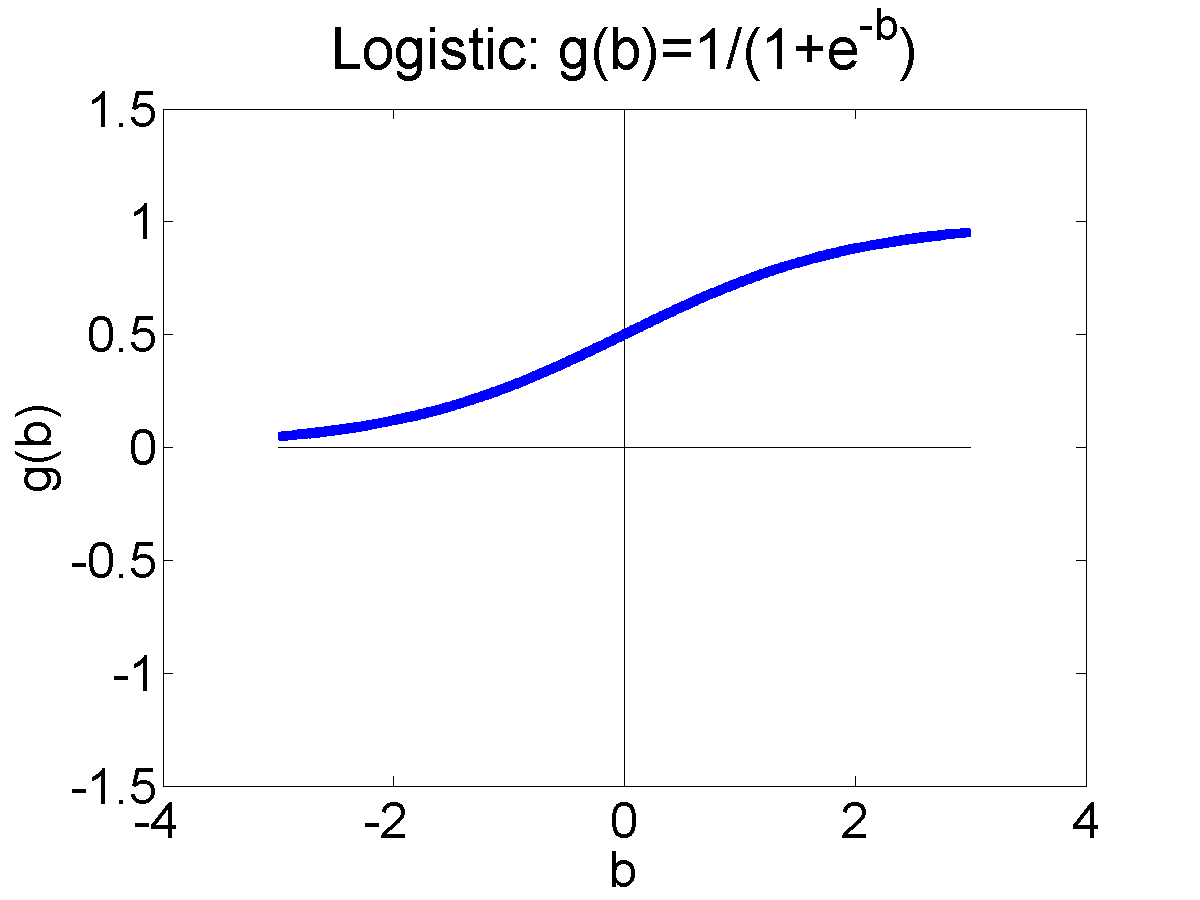
\includegraphics[width=1.75in]{figs/nn_logistic.png}}
    \end{block}
    \column{2.25in}
    \begin{block}{Why to use the logistic function}
      \[
      \sigma(z) = \begin{cases}
        1 & z\rightarrow\infty\\
        0 & z\rightarrow -\infty\\
        \mbox{in between} & \mbox{in between}
      \end{cases}
      \]
      and $\sigma(z)$ is smoothly differentiable, so we can use
      gradient descent for training.
    \end{block}
  \end{columns}
\end{frame}

\begin{frame}
  \frametitle{Derivative of a sigmoid}
  The derivative of a sigmoid is pretty easy to calculate:
  \[
  \sigma(z)=\frac{1}{1+e^{-z}},~~~\frac{d\sigma}{dz}=\frac{e^{-z}}{(1+e^{-z})^2}
  \]
  An interesting fact that's extremely useful, in computing back-prop,
  is that we can write the derivative in terms
  of $\sigma(z)$, without any need to store $z$:
  \begin{align*}
    \frac{d\sigma}{dz} &=\frac{e^{-z}}{(1+e^{-z})^2}\\
    &=\left(\frac{1}{1+e^{-z}}\right)\left(\frac{e^{-z}}{1+e^{-z}}\right)\\
    &=\left(\frac{1}{1+e^{-z}}\right)\left(1-\frac{1}{1+e^{-z}}\right)\\
    &=\sigma(z)(1-\sigma(z))
  \end{align*}
\end{frame}

\begin{frame}
  \begin{columns}[t]
    \column{2.25in}
    \begin{block}{Step function and its derivative}
      \centerline{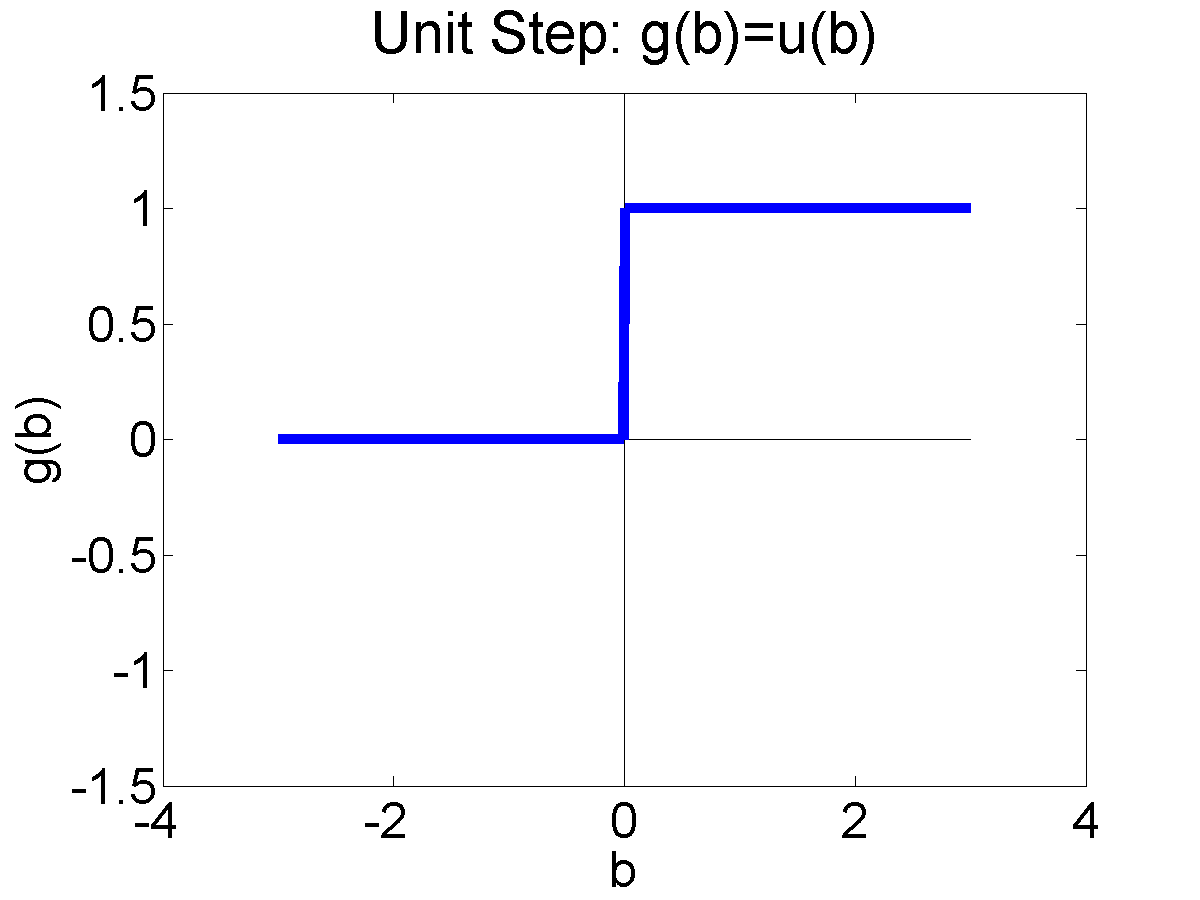
\includegraphics[width=1.75in]{figs/nn_unitstep.png}}
      \begin{itemize}
      \item The derivative of the step function is the Dirac
        delta, which is not very useful in gradient descent
      \end{itemize}
    \end{block}
    \column{2.25in}
    \begin{block}{Logistic function and its derivative}
      \centerline{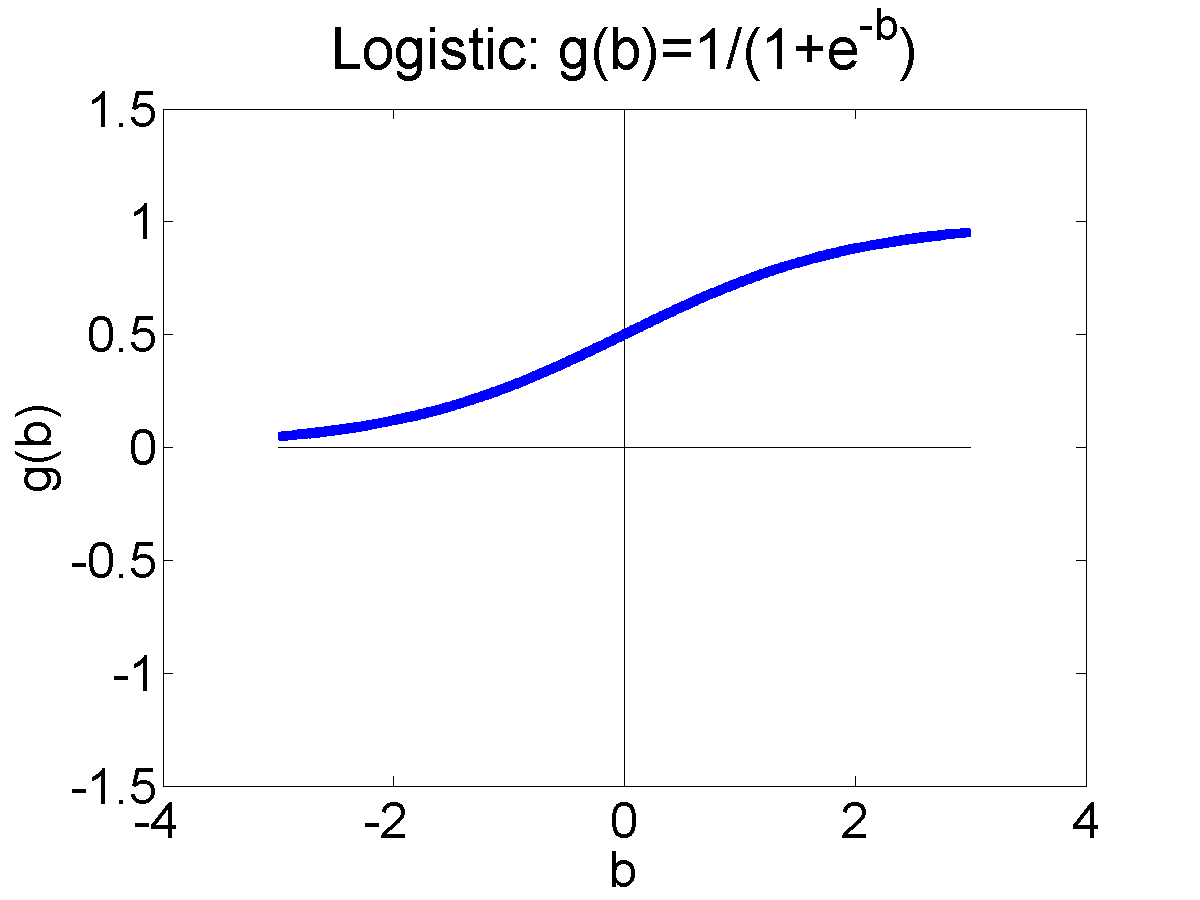
\includegraphics[width=1.75in]{figs/nn_logistic.png}}
      \centerline{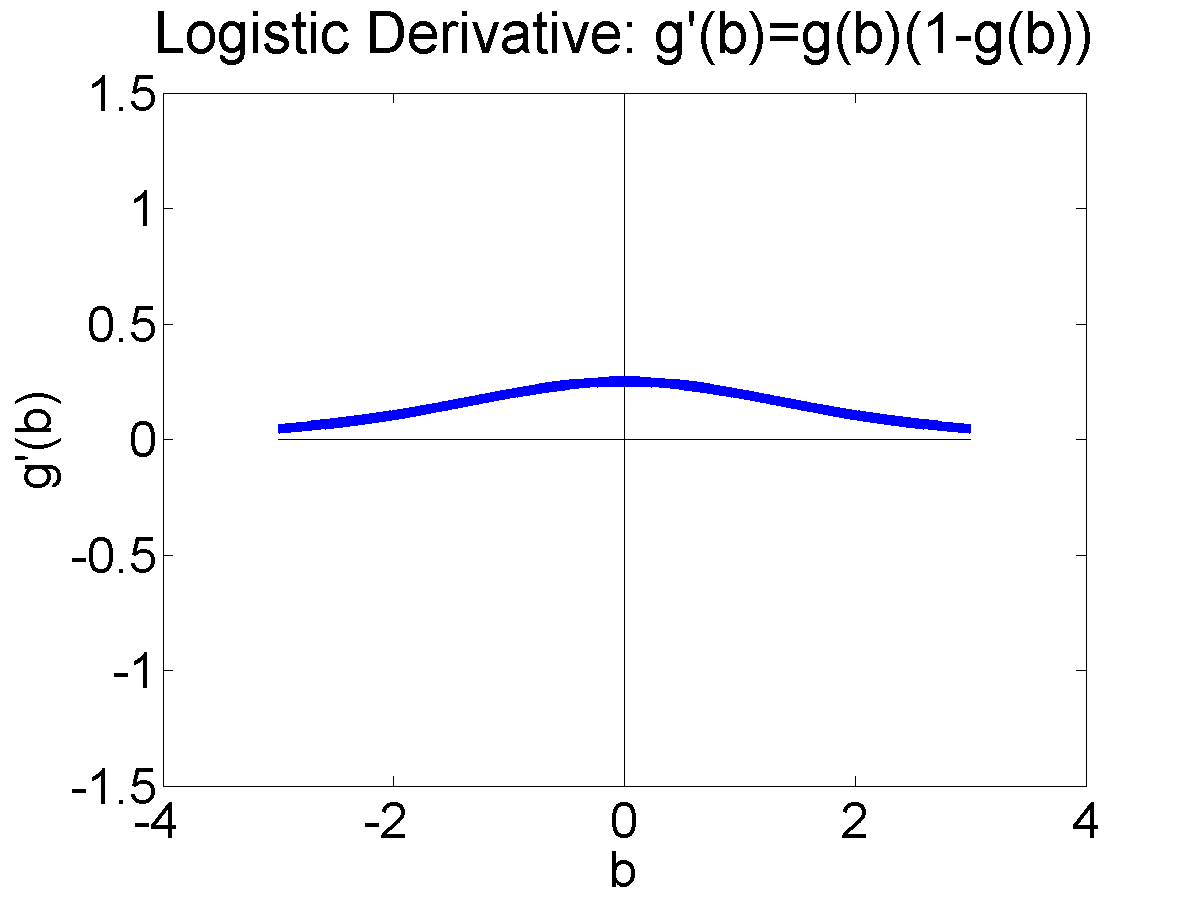
\includegraphics[width=1.75in]{figs/nn_logisticprime.png}}
    \end{block}
  \end{columns}
\end{frame}

\begin{frame}
  \frametitle{Signum and Tanh}

  The signum function is like the unit step, but two-sided.  It is
  used if, for some reason, you want your output to be
  $y\in\left\{-1,1\right\}$, instead of $y\in\left\{0,1\right\}$:
  \[
  \mbox{sign}(z)=\begin{cases}
  -1 & z<0\\
  1 & z>0
  \end{cases}
  \]
  It is usually approximated by the hyperbolic tangent function
  (tanh), which is just a scaled shifted version of the sigmoid:
  \begin{displaymath}
    \tanh(z) = \frac{e^z-e^{-z}}{e^z+e^{-z}}
    = \frac{1-e^{-2z}}{1+e^{-2z}}
    = 2\sigma(2z)-1
  \end{displaymath}
  and which has a scaled version of the sigmoid derivative:
  \begin{align*}
    \frac{d\tanh(z)}{dz} =\left(1-\tanh^2(z)\right)
  \end{align*}
\end{frame}

\begin{frame}
  \begin{columns}[t]
    \column{2.25in}
    \begin{block}{Signum function and its derivative}
      \centerline{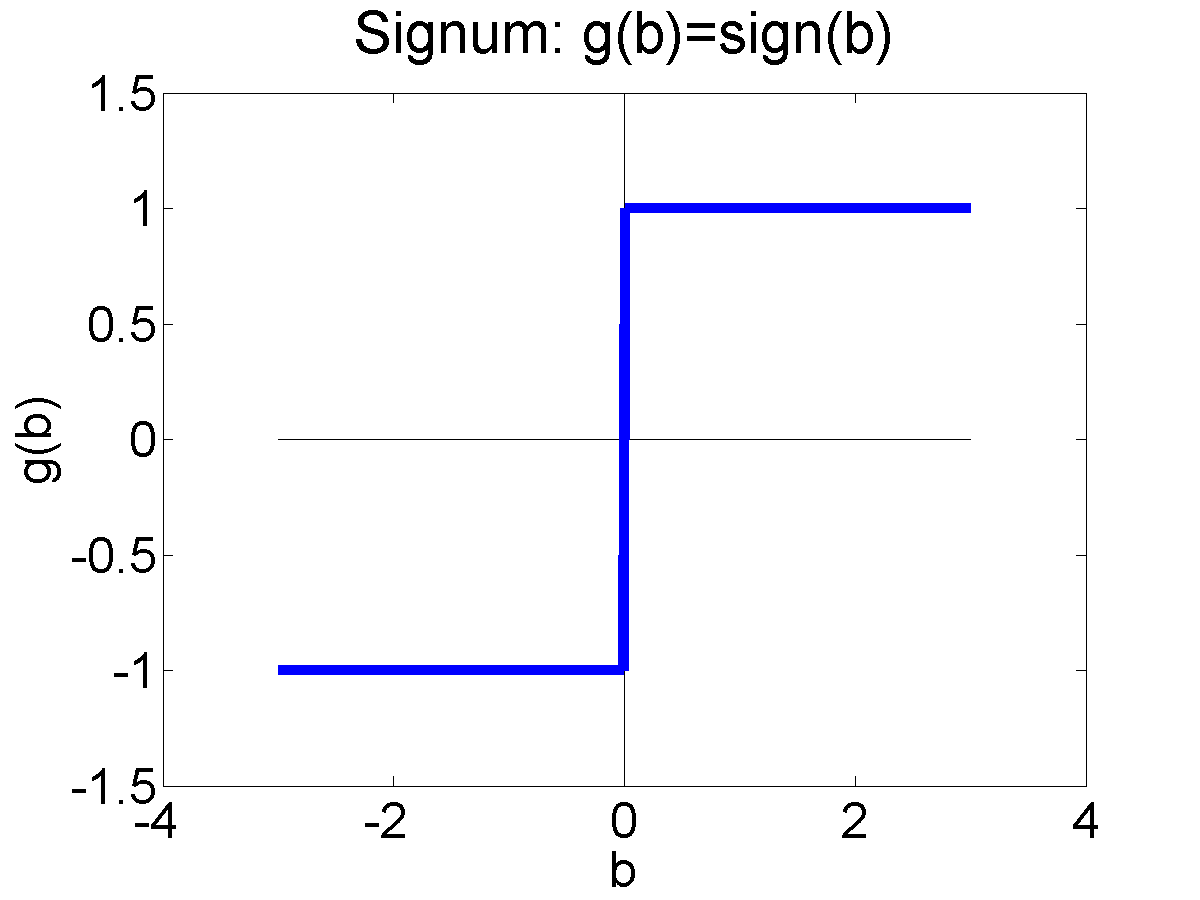
\includegraphics[width=1.75in]{figs/nn_signum.png}}
      \begin{itemize}
      \item The derivative of the signum function is $2\delta(z)$,
         which is not very useful in gradient descent.
      \end{itemize}
    \end{block}
    \column{2.25in}
    \begin{block}{Tanh function and its derivative}
      \centerline{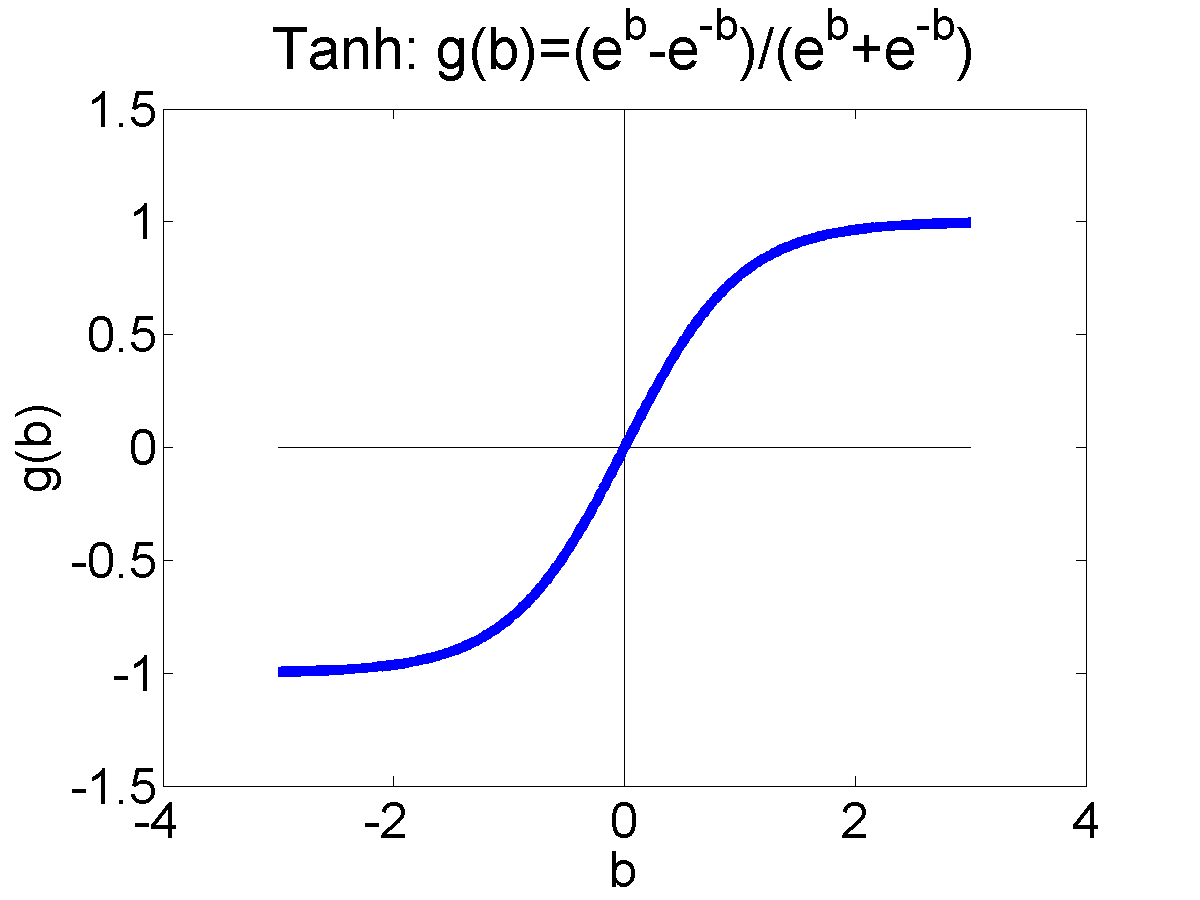
\includegraphics[width=1.75in]{figs/nn_tanh.png}}
      \centerline{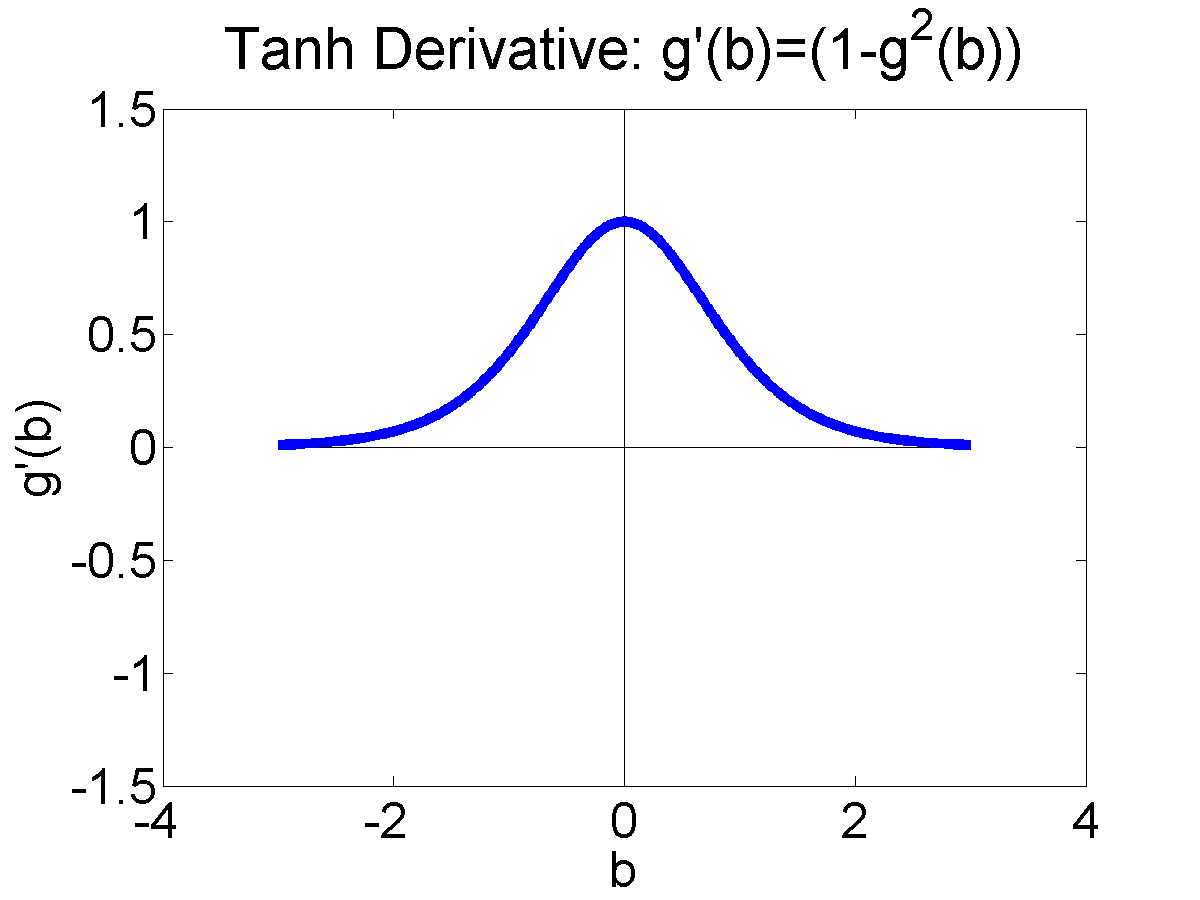
\includegraphics[width=1.75in]{figs/nn_tanhprime.png}}
    \end{block}
  \end{columns}
\end{frame}

\begin{frame}
  \centerline{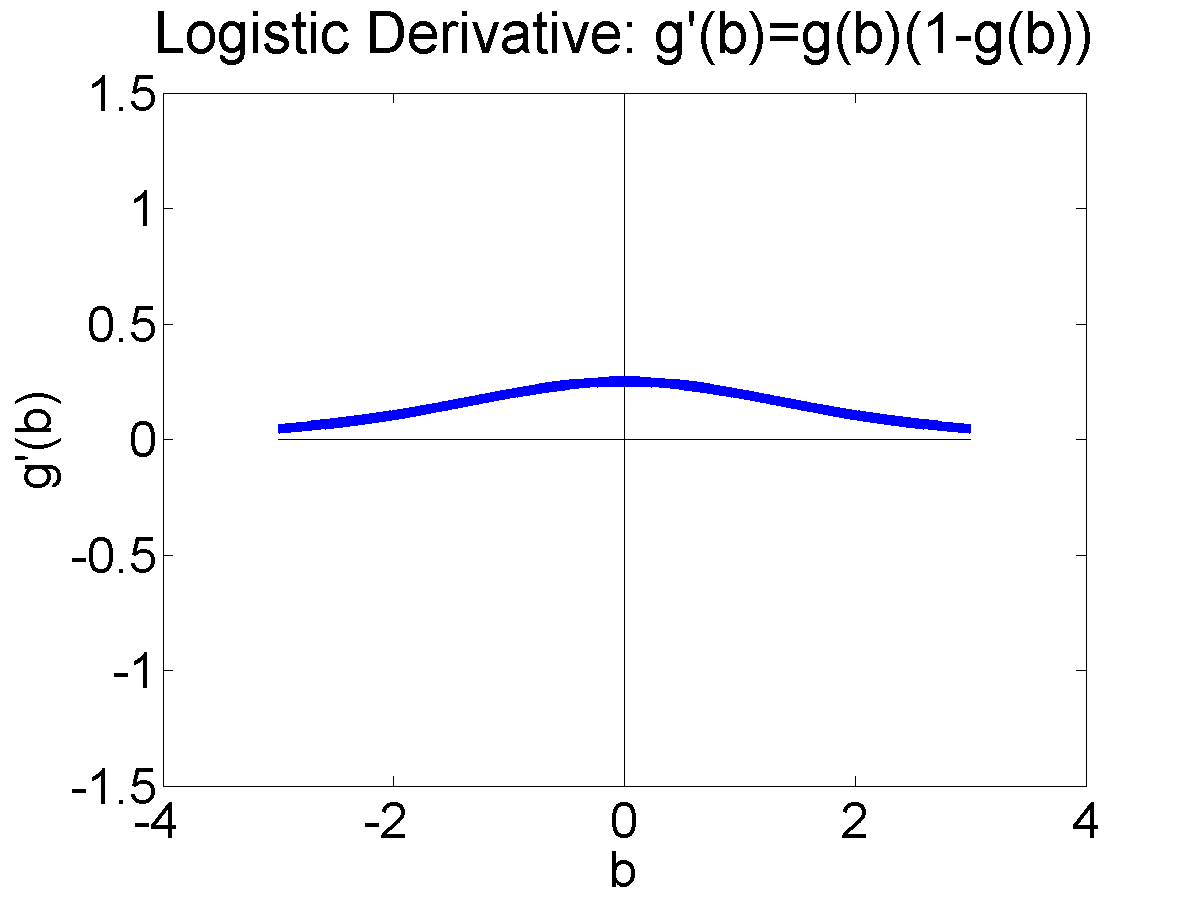
\includegraphics[width=1in]{figs/nn_logisticprime.png}}
  
  The sigmoid has a surprising problem: for large values of $w$,
  $\frac{\partial\sigma(wx)}{\partial{w}}\rightarrow 0$.
  \begin{itemize}
  \item When we begin training, we start with small values of $w$.
    $\frac{\partial\sigma(wx)}{\partial w}$ is
    reasonably large, so gradient descent works well for training.
  \item If we have lots of training tokens with similar target values,
    then the gradient ($\frac{\partial\mathcal{L}}{\partial{w}}$) is
    similar for all of them.  Gradient descent adds up many of these
    values as $w\leftarrow
    w-\frac{\partial{\mathcal{L}}}{\partial{w}}$. After a few such
    examples, $w$ gets very large.  At that point,
    $\frac{\partial\sigma(wx)}{\partial{w}}\rightarrow 0$, and
    training effectively stops.
  \item After that point, even if the neural net sees new training
    data that don't match what it has already learned, it can no
    longer change.  We say that it has suffered from the ``vanishing
    gradient problem.''
  \end{itemize}
\end{frame}
    
\begin{frame}
  \frametitle{A solution to the vanishing gradient problem: ReLU}
  \centerline{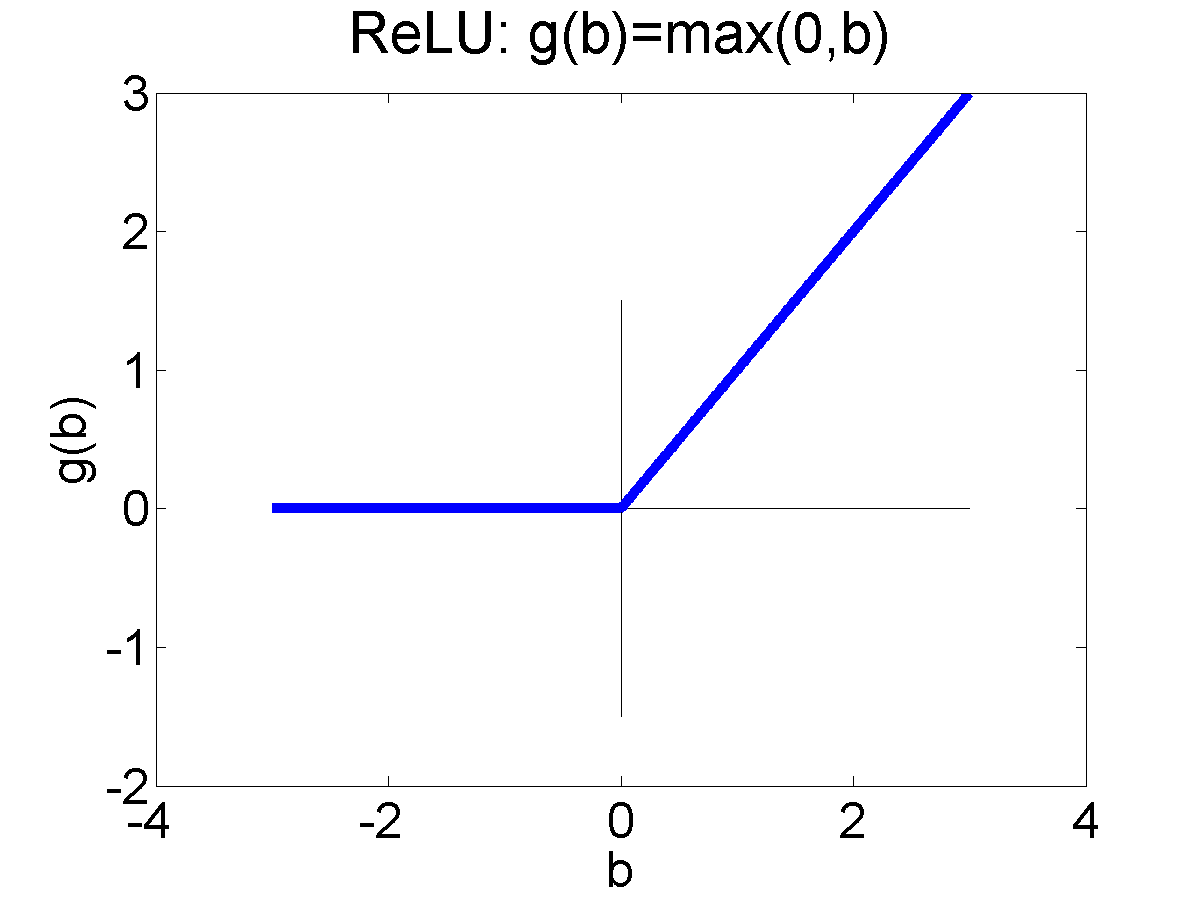
\includegraphics[width=1in]{figs/nn_relu.png}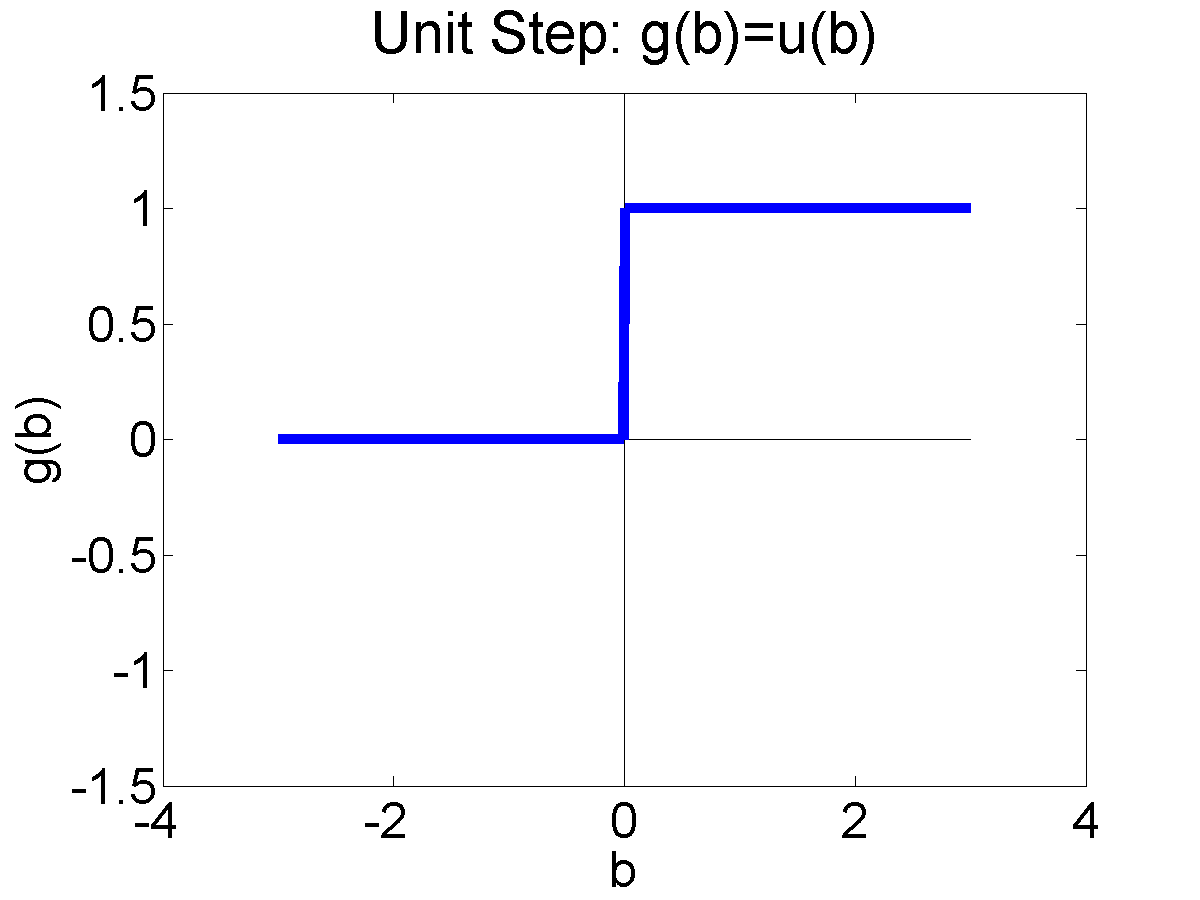
\includegraphics[width=1in]{figs/nn_unitstep.png}}

  The most ubiquitous solution to the vanishing gradient problem is to
  use a ReLU (rectified linear unit) instead of a sigmoid.  The ReLU
  is given by
  \[
  \mbox{ReLU}(z) = \begin{cases}
    z & z\ge 0\\
    0 & z\le 0,
  \end{cases}
  \]
  and its derivative is the unit step.  Notice that the
  unit step is equally large ($u(wx)=1$)  for any positive value ($wx>0$), so
  no matter how large $w$ gets, back-propagation continues to work.
\end{frame}

\begin{frame}
  \frametitle{A solution to the vanishing gradient problem: ReLU}
  \centerline{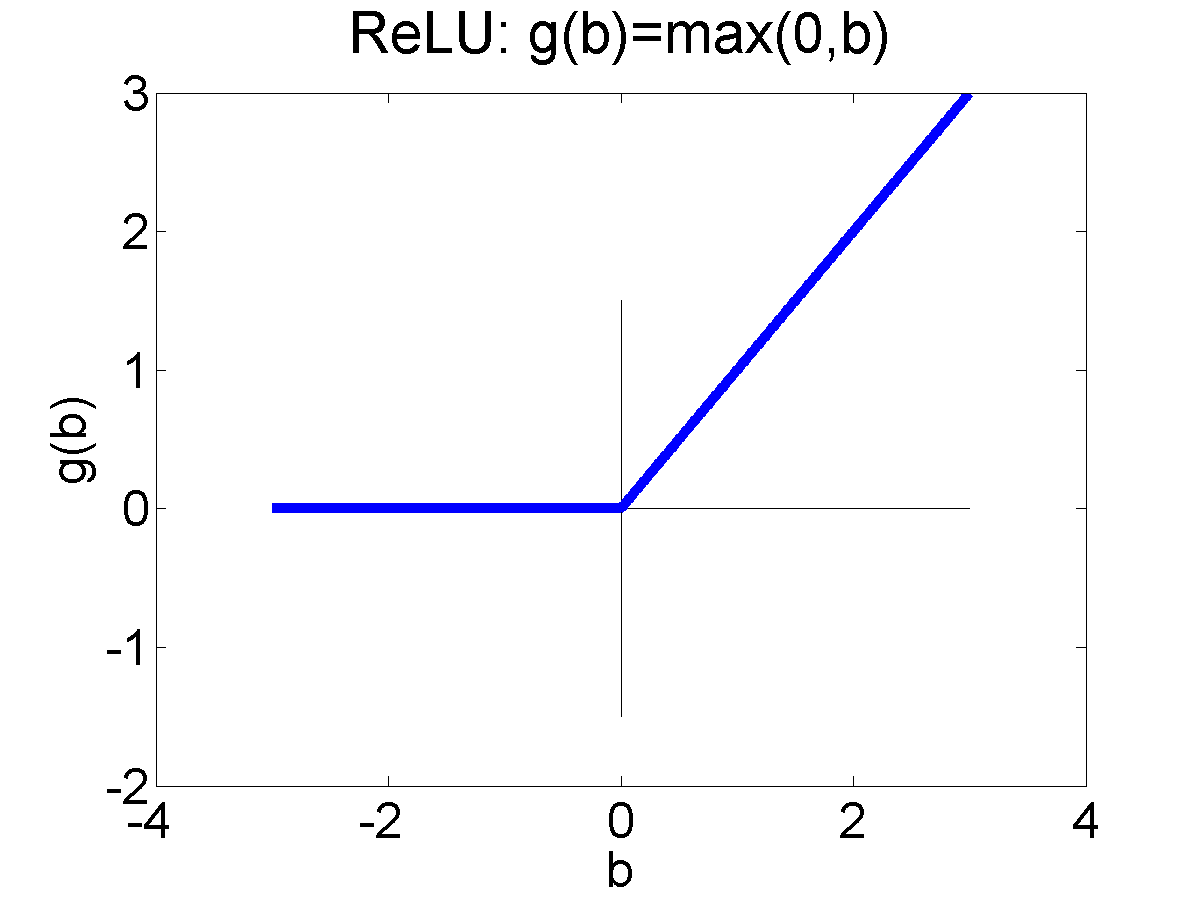
\includegraphics[width=1in]{figs/nn_relu.png}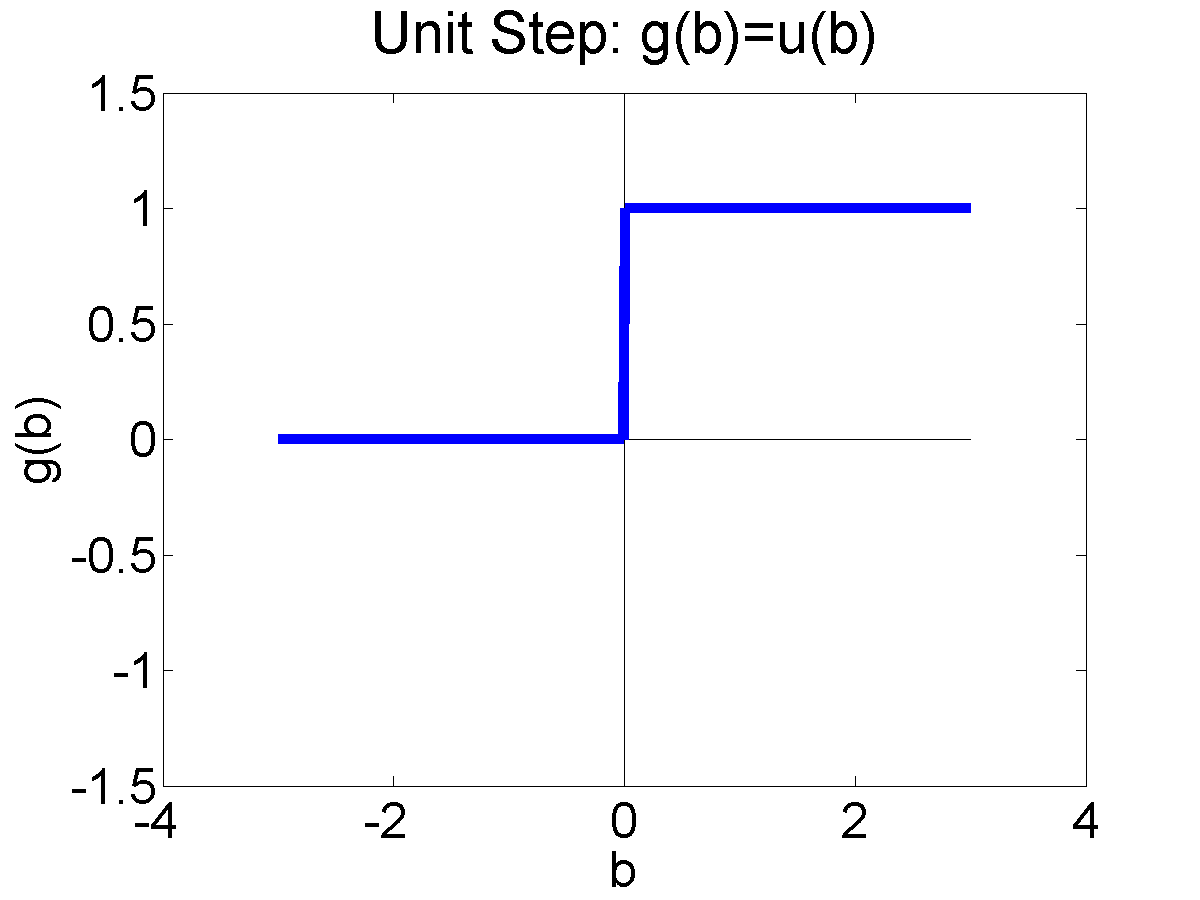
\includegraphics[width=1in]{figs/nn_unitstep.png}}

  \begin{itemize}
    \item {\bf Pro:} The ReLU derivative is equally large
      ($\frac{d\mbox{ReLU}(wx)}{d(wx)}=1$) for any positive value
      ($wx>0$), so no matter how large $w$ gets, back-propagation
      continues to work.
    \item {\bf Con:} If the ReLU is used as a hidden unit
      ($a_j=\mbox{ReLU}(z_j)$), then your output is no longer a
      piece-wise constant approximation of $\mathbf{y}$.  It is now
      piece-wise linear.
    \item On the other hand, maybe piece-wise linear is
      better than piece-wise constant, so\ldots
  \end{itemize}
\end{frame}
      
\begin{frame}
  \frametitle{A solution to the vanishing gradient problem: the ReLU}
  \centerline{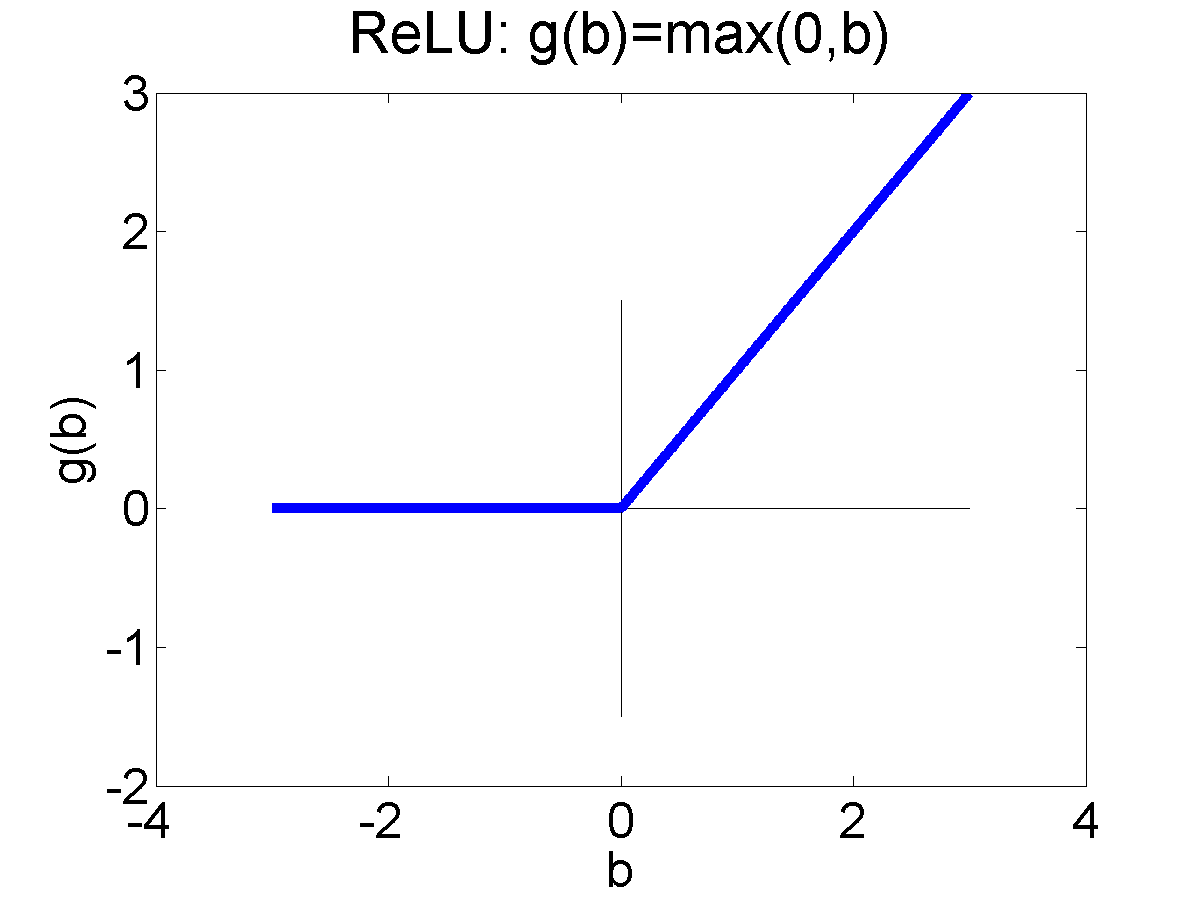
\includegraphics[width=1in]{figs/nn_relu.png}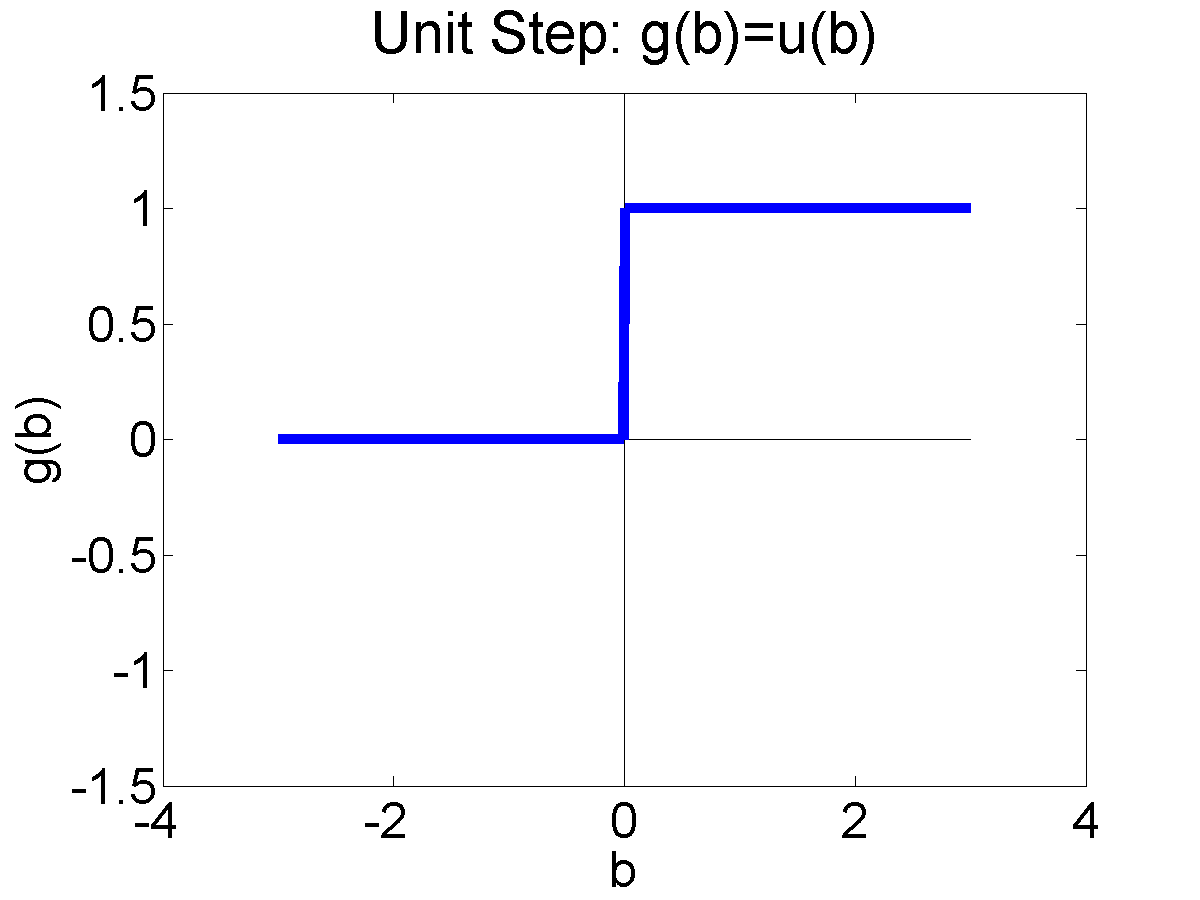
\includegraphics[width=1in]{figs/nn_unitstep.png}}

  \begin{itemize}
    \item {\bf Pro:} The ReLU derivative is equally large
      ($\frac{d\mbox{ReLU}(wx)}{d(wx)}=1$) for any positive value
      ($wx>0$), so no matter how large $w$ gets, back-propagation
      continues to work.
    \item {\bf Pro:} If the ReLU is used as a hidden unit
      ($a_j=\mbox{ReLU}(z_j)$), then your output is no longer a
      piece-wise constant approximation of $\mathbf{y}$.  It is now
      piece-wise linear.
    \item {\bf Con:} ??
  \end{itemize}
\end{frame}

\begin{frame}
  \frametitle{The dying ReLU problem}
  \centerline{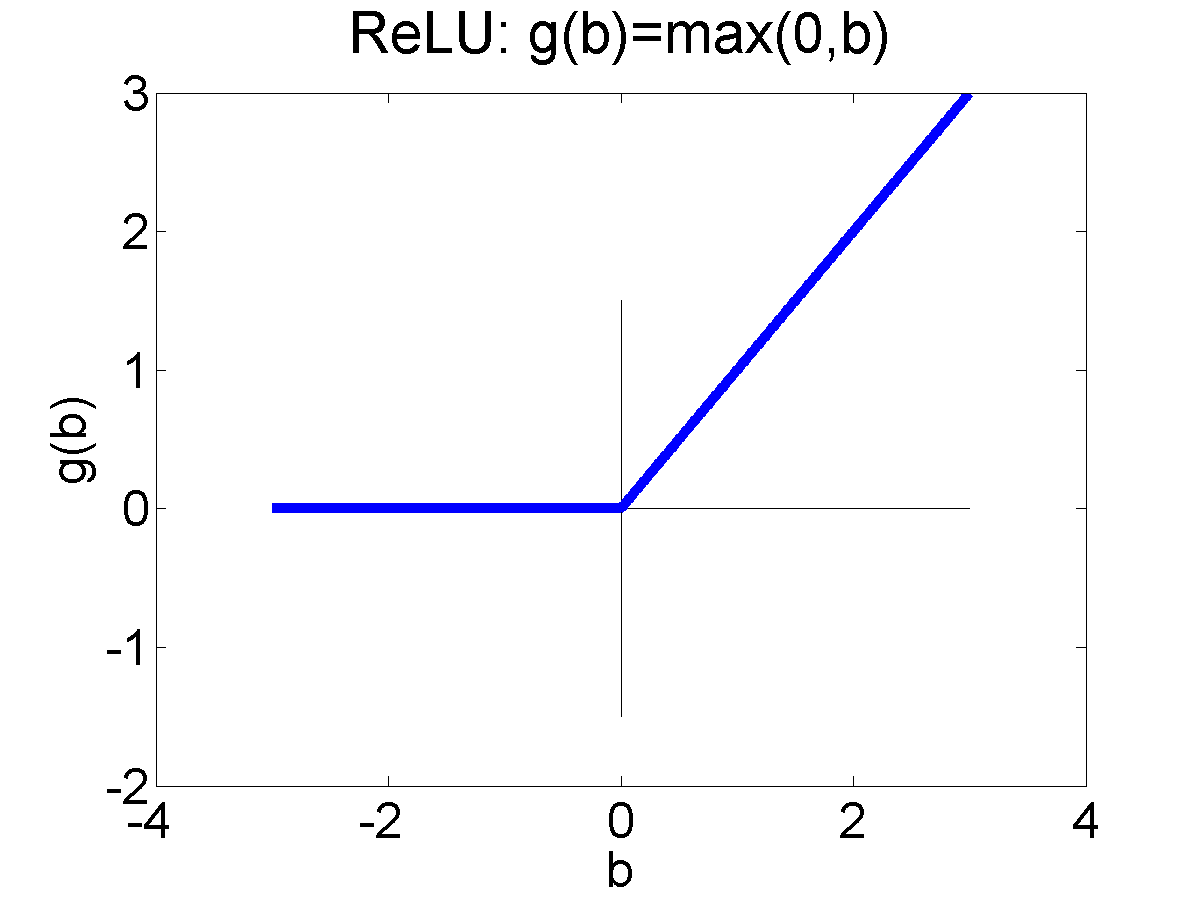
\includegraphics[width=1in]{figs/nn_relu.png}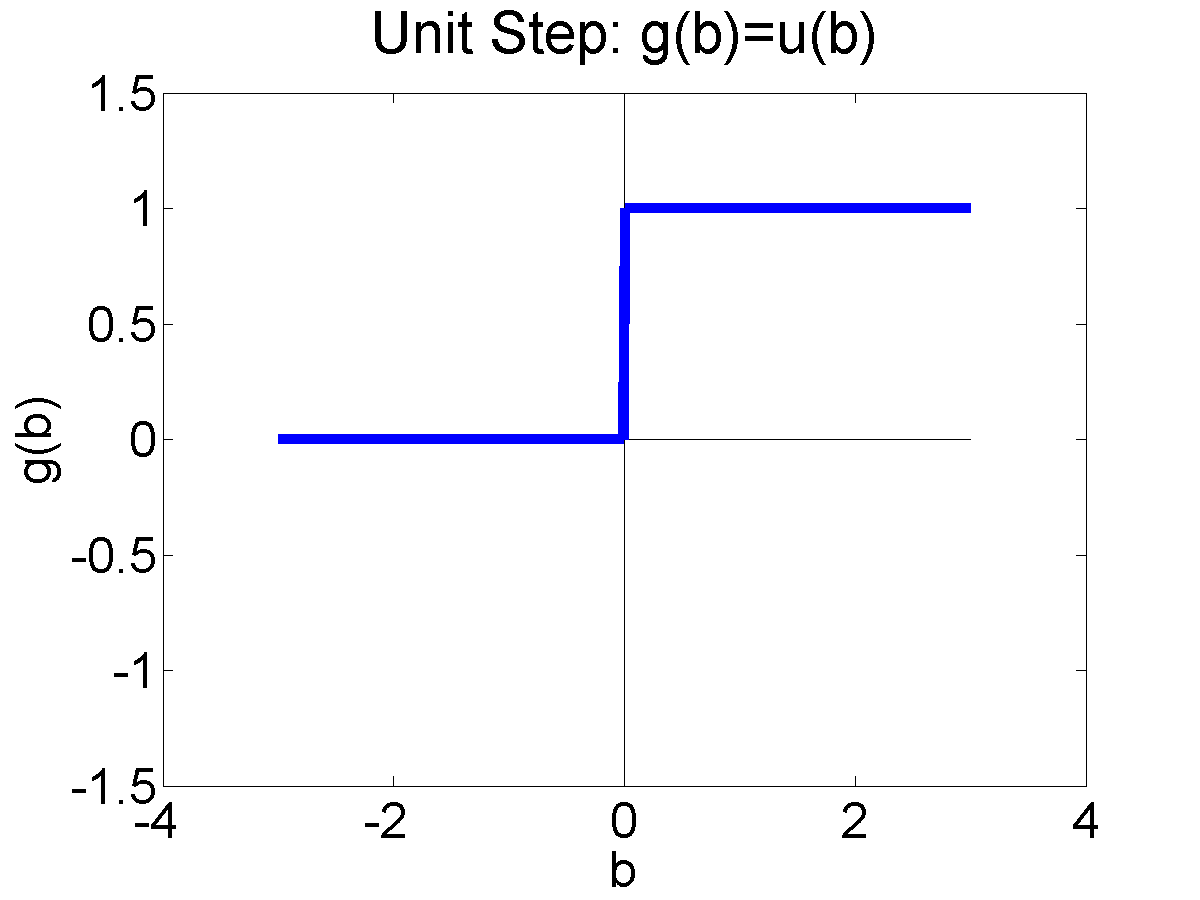
\includegraphics[width=1in]{figs/nn_unitstep.png}}

  \begin{itemize}
    \item {\bf Pro:} The ReLU derivative is equally large
      ($\frac{d\mbox{ReLU}(wx)}{d(wx)}=1$) for any positive value
      ($wx>0$), so no matter how large $w$ gets, back-propagation
      continues to work.
    \item {\bf Pro:} If the ReLU is used as a hidden unit
      ($a_j=\mbox{ReLU}(z_j)$), then your output is no longer a
      piece-wise constant approximation of $\mathbf{y}$.  It is now
      piece-wise linear.
    \item {\bf Con:} If $wx+b<0$, then
      ($\frac{d\mbox{ReLU}(wx)}{d(wx)}=0$), and learning stops.
      In the worst case, if $b$ becomes very negative, then all of the
      hidden nodes are turned off---the network computes nothing, and
      no learning can take place!  This is called the ``Dying ReLU
      problem.''
  \end{itemize}
\end{frame}

\begin{frame}
  \frametitle{Solutions to the Dying ReLU problem}

  \begin{itemize}
  \item {\bf Softplus:}  Pro: always positive.  Con: gradient$\rightarrow 0$ as $x\rightarrow -\infty$.
    \[
    f(x) = \ln\left(1+e^x\right)
    \]
  \item {\bf Leaky ReLU:} Pro: gradient constant, output piece-wise linear.  Con:
    negative part might fail to match your dataset.
    \[
    f(x) = \begin{cases}
      x & x \ge 0\\
      0.01x & x \le 0
    \end{cases}
    \]
  \item {\bf Parametric ReLU (PReLU:)} Pro: gradient constant, ouput
    PWL.  The slope of the negative part ($a$) is a trainable
    parameter, so can adapt to your dataset.  Con: you have to train it.
    \[
    f(x) = \begin{cases}
      x & x \ge 0\\
      ax & x \le 0
    \end{cases}
    \]
  \end{itemize}
\end{frame}

%%%%%%%%%%%%%%%%%%%%%%%%%%%%%%%%%%%%%%%%%%%%%
\section[Loss]{Loss Functions}
\setcounter{subsection}{1}

\begin{frame}
  \frametitle{How to train a neural network}
  \begin{enumerate}
  \item Find a {\bf training dataset} that contains $n$ examples showing the
    desired output, $\mathbf{y}_i$, that the NN should compute in
    response to input vector $\mathbf{x}_i$:
    \[
      {\mathcal D}=\left\{(\mathbf{x}_1,\mathbf{y}_1),\ldots,(\mathbf{x}_n,\mathbf{y}_n)\right\}
    \]
    \item Randomly {\bf initialize} $\mathbf{W}_{1}$,
      $\mathbf{b}_{1}$, $\mathbf{W}_{2}$, and $\mathbf{b}_{2}$.
    \item Perform {\bf forward propagation}: find out what the neural
      net computes as $\mathbf{g}(\mathbf{x}_i)$ for each $\mathbf{x}_i$.
    \item Define a {\bf loss function} that measures
      how badly $\mathbf{g}(\mathbf{x}_i)$ differs from $\mathbf{y}_i$.
    \item Perform {\bf back propagation} to find the derivatives of the loss w.r.t.  $\mathbf{a}_{1}$,
      $\mathbf{z}_{1}$, $\mathbf{a}_{2}$, and $\mathbf{z}_{2}$.
    \item Calculate the {\bf loss gradients}
      $\frac{\partial\mathcal{L}}{\partial\mathbf{W}_{1}}$,
      $\frac{\partial\mathcal{L}}{\partial\mathbf{b}_{1}}$,
      $\frac{\partial\mathcal{L}}{\partial\mathbf{W}_{2}}$, and
      $\frac{\partial\mathcal{L}}{\partial\mathbf{b}_{2}}$.
    \item Perform {\bf gradient descent} to improve  $\mathbf{W}_{1}$,
      $\mathbf{b}_{1}$, $\mathbf{W}_{2}$, and $\mathbf{b}_{2}$.
    \item Repeat steps 3-6 until convergence.
  \end{enumerate}
\end{frame}

\begin{frame}
  \frametitle{Loss Functions in General: Probability}

  \begin{itemize}
  \item 
    We want $\mathbf{g}(\mathbf{x})$ to give us as much information as
    possible about $\mathbf{y}$.  We formalize that by interpreting
    $\mathbf{g}(\mathbf{x})$ as some kind of probability model, and by
    maximizing $\Pr(\mathbf{y}|\mathbf{g}(\mathbf{x}))$.
  \item
    If we assume the training examples are independent, then it
    makes sense to multiply their probabilities. 
    \begin{align*}
      \Pr\left(\mathcal{D}\right) &= \prod_{i=1}^n \Pr\left(\mathbf{y}_i|\mathbf{x}_i\right)
    \end{align*}
  \end{itemize}
\end{frame}

\begin{frame}
  \frametitle{Loss Functions in General: Negative Log Probability}

  \begin{itemize}
  \item 
    Adding log
    probabilities is much easier than multiplying probabilities.
    \begin{align*}
      \Pr\left(\mathcal{D}\right) &= \prod_{i=1}^n \Pr\left(\mathbf{y}_i|\mathbf{x}_i\right)\\
      \ln\Pr\left(\mathcal{D}\right) &= \sum_{i=1}^n \ln\Pr\left(\mathbf{y}_i|\mathbf{x}_i\right)
    \end{align*}
  \item
    ``Minimizing the loss'' is the same thing as ``maximizing the
    log probability'' if we set the ``loss'' (${\mathcal L}$) equal
    to the average negative log probability.  We will often use
    $E\left[\cdot\right]$ to mean ``average value:''
    \begin{align*}
      \mathcal{L}=E\left[-\ln\Pr(\mathbf{y}|\mathbf{x})\right]=
      -\frac{1}{n}\sum_{i=1}^n\Pr(\mathbf{y}_i|\mathbf{x}_i)
    \end{align*}
  \end{itemize}
\end{frame}

\begin{frame}
  \frametitle{Loss Function: Binary Classifier}

  \centerline{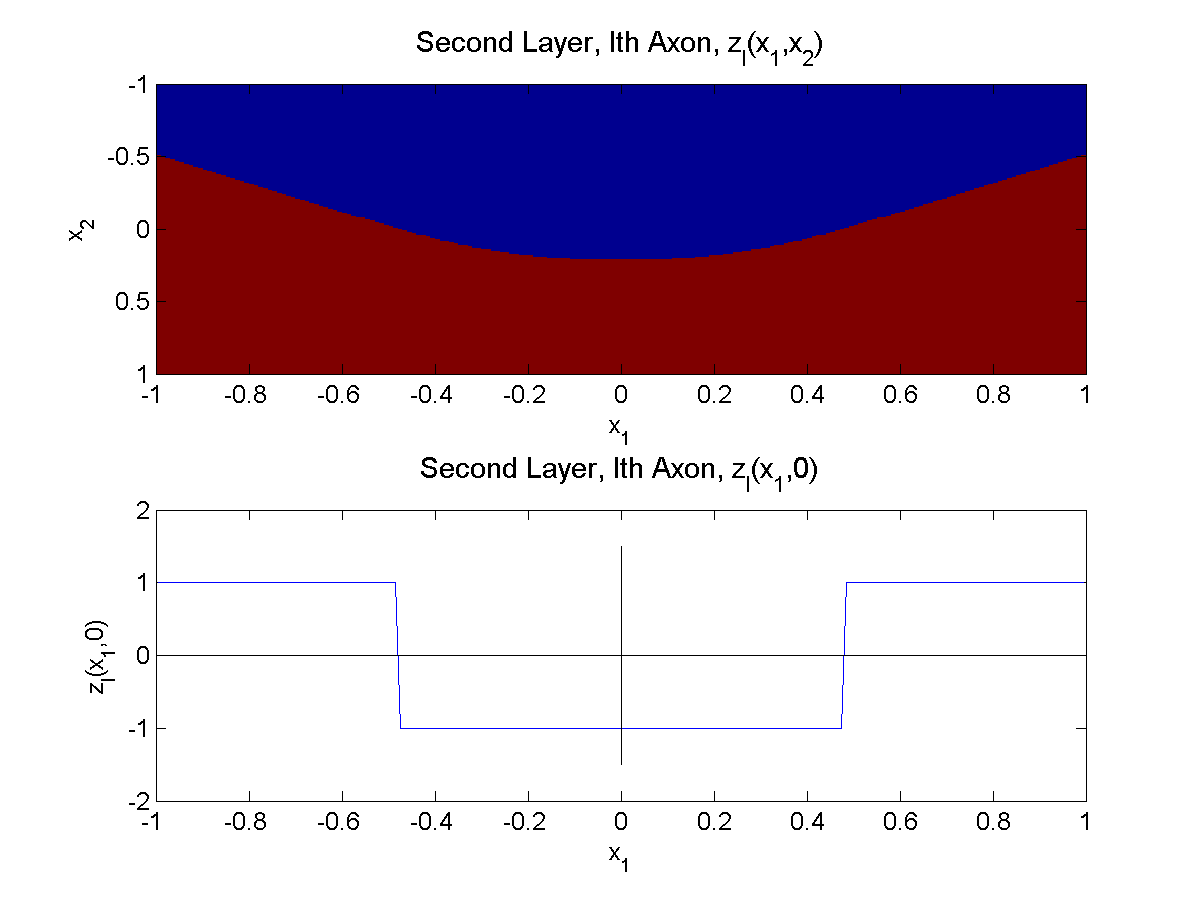
\includegraphics[width=3in]{figs/nn_axon2.png}}

  For a binary classifier, the target output is binary, $y\in\{0,1\}$.
  Suppose we interpret this as the observed value of a Bernoulli
  random variable, $Y$.
\end{frame}
\begin{frame}
  \frametitle{Loss Function: Binary Classifier}
  Suppose we use a
  sigmoid output nonlinearity, so that $0<g(\mathbf{x})<1$, then we
  can interpret $g(\mathbf{x})$ as the probability that $Y$ should be
  one:
  \begin{displaymath}
    g(\mathbf{x}) = \Pr(Y=1|\mathbf{x})
  \end{displaymath}
  Under this interpretation, the loss function is
  \begin{align*}
    \mathcal{L}
    &= E\left[-\ln\Pr(Y=y|\mathbf{x})\right]\\
    &= -E\left[y\ln\Pr(Y=1|\mathbf{x|})+(1-y)\ln\Pr(Y=0|\mathbf{x})\right]\\
    &= -E\left[y\ln g(\mathbf{x})+(1-y)\ln(1-g(\mathbf{x}))\right]
  \end{align*}
\end{frame}


\begin{frame}
  \frametitle{Loss Function: Multinomial Classifier}

  \centerline{\includegraphics[width=1in]{exp/voronoi.png}}
  {\footnotesize\url{https://commons.wikimedia.org/wiki/File:Euclidean_Voronoi_diagram.svg}}
  
  The best way to formulate an $m$-class classifier is by having an
  $m$-element {\bf one-hot} output vector, $\mathbf{y}\in\{0,1\}^m$,
  where
  \begin{displaymath}
    y_k=\begin{cases}
    1 & k~\text{is the correct class}\\
    0 & \mbox{otherwise}
    \end{cases}
  \end{displaymath}
\end{frame}

\begin{frame}
  \frametitle{Loss Function: Multinomial Classifier}
  
  \centerline{\includegraphics[width=1in]{exp/voronoi.png}}
  
  Now we want the neural net output,
  $\mathbf{g}(\mathbf{x})=[g_1(\mathbf{x}),g_2(\mathbf{x}),\ldots]^T$,
  to be interpretable as a set of probabilities,
  $g_k(\mathbf{x})=\Pr(Y_k=1|\mathbf{x})$.  In order to be interpreted
  as probabilities, the outputs need to satisfy: $0\le
  g_k(\mathbf{x})\le 1$ and $\sum_{k} g_k(\mathbf{x})=1$.  An
  output nonlinearity that satisfies these conditions is the {\bf
    softmax}, defined as
  \begin{displaymath}
    g_k(\mathbf{x}) = \softmax_k(\mathbf{z}_2) =
    \frac{e^{z_{2,k}}}{\sum_{k'} e^{z_{2,k'}}}
  \end{displaymath}
\end{frame}
    
\begin{frame}
  \frametitle{Loss Function: Multinomial Classifier}

  We can interpret
  $g_k(\mathbf{x})=\Pr(Y_k=1|\mathbf{x})$ if
  \begin{displaymath}
    Y_k=\begin{cases}
    1 & k~\text{is the correct class}\\
    0 & \mbox{otherwise}
    \end{cases},~~~~
    g_k(\mathbf{x}) = \frac{e^{z_{2,k}}}{\sum_{k'} e^{z_{2,k'}}}
  \end{displaymath}
  With these definitions, the loss function is the {\bf cross-entropy loss}:
  \begin{align*}
    \mathcal{L}
    &= E\left[-\ln\Pr(\mathbf{y}|\mathbf{x})\right]\\
    &= -E\left[\sum_k y_k\ln g_k(\mathbf{x})\right]\\
    &= -\frac{1}{n}\sum_{i=1}^n \ln g_{\text{correct class}}(\mathbf{x}_i)
  \end{align*}
\end{frame}

\begin{frame}
  \frametitle{Loss Function: Regression}

  For a nonlinear regression neural net, the target function
  $\mathbf{y}$ is an arbitrary real vector.  In this case, a useful
  probability model assumes that
  \begin{displaymath}
    \mathbf{y}=\mathbf{g}(\mathbf{x})+\mathbf{v},
  \end{displaymath}
  where $\mathbf{v}$ is zero-mean, unit variance Gaussian noise:
  \begin{align*}
    \Pr(\mathbf{y}|\mathbf{g}(\mathbf{x}))=
    e^{-\frac{1}{2}\Vert\mathbf{y}-\mathbf{g}(\mathbf{x})\Vert^2}
  \end{align*}
  The loss function is then just the mean squared error:
  \begin{align*}
    \mathcal{L}
    &= E\left[-\ln\Pr(\mathbf{y}|\mathbf{x})\right]\\
    &= E\left[\frac{1}{2}\Vert\mathbf{y}-\mathbf{g}(\mathbf{x})\Vert^2\right]\\
    &= -\frac{1}{2n}\sum_{i=1}^n\Vert\mathbf{y}_i-\mathbf{g}(\mathbf{x}_i)\Vert^2
  \end{align*}
\end{frame}
  
\begin{frame}
  \frametitle{Loss Function: Regression}
  \begin{block}{Minimum Mean Squared Error (MMSE)$\Rightarrow$ $\mathbf{g}(\mathbf{x})=$ conditional expected value of $\mathbf{y}$}
    \[
    \mathbf{g}^*(\mathbf{x})=\argmin {\mathcal L} = 
    \argmin\frac{1}{2}E\left[\Vert\mathbf{y}-\mathbf{g}(\mathbf{x})\Vert^2\right]
    \]
    which is minimized by
    \[
    \mathbf{g}_{MMSE}(\mathbf{x})=E\left[\mathbf{y}|\mathbf{x}\right]
    \]
  \end{block}
\end{frame}

%%%%%%%%%%%%%%%%%%%%%%%%%%%%%%%%%%%%%%%%%%%%%
\section[Learning]{Learning: Gradient Descent}
\setcounter{subsection}{1}

\begin{frame}
  \frametitle{Gradient Descent: How do we improve $\mathbf{W}$ and $\mathbf{b}$?}  Given
  some initial neural net parameter
  we want to find a better value of the same parameter.  We do that
  using gradient descent:
  \[
  \mathbf{W}\leftarrow \mathbf{W}-\eta\left(\frac{\partial{\mathcal L}}{\partial\mathbf{W}}\right)^T,
  \]
  where $\eta$ is a learning rate (some small constant, e.g., $\eta=0.001$ or so).
  \centerline{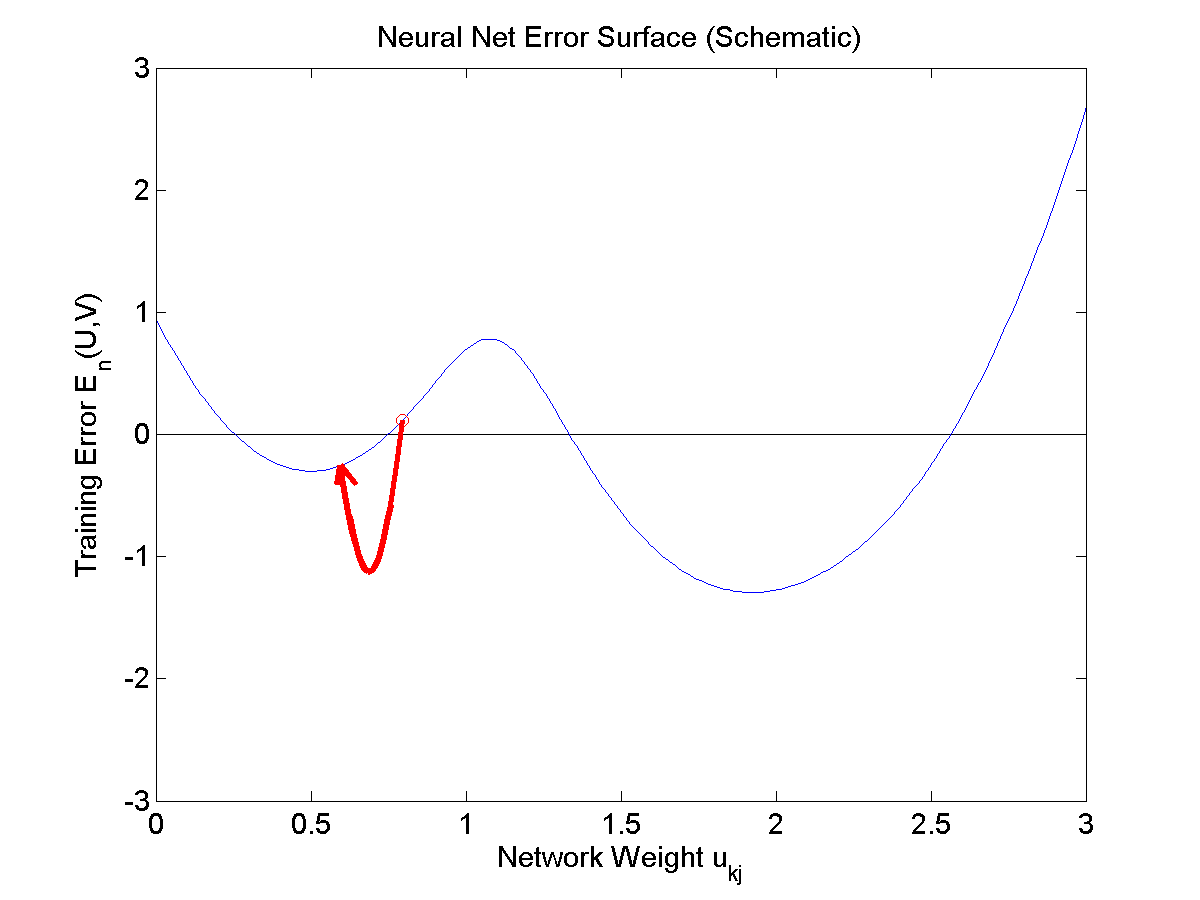
\includegraphics[width=2in]{figs/nn_errorsurf1.png}}
\end{frame}


\begin{frame}
  \frametitle{Loss Gradient}

  Suppose we use MSE loss:
  \begin{align*}
    \mathcal{L} =E\left[\Vert\mathbf{y}-\mathbf{g}(\mathbf{x})\Vert^2\right]
    =E\left[\Vert\mathbf{y}-\mathbf{a}_2(\mathbf{x})\Vert^2\right],
  \end{align*}
  where the expectation means ``average over the training data.''
  Since $\mathcal{L}$ is a scalar, it should be possible to compute
  $\frac{\partial\mathcal{L}}{\partial\mathbf{W}_l}$, but how?  For
  example, can we use the chain rule?  Let's try:
  \begin{displaymath}
    \mathbf{a}_2 = f_2\left(\mathbf{z}_2\right),~~~
    \mathbf{z}_2=\mathbf{b}_2+\mathbf{W}_2\mathbf{a}_1
  \end{displaymath}
  \begin{displaymath}
    \frac{\partial\mathcal{L}}{\partial\mathbf{W}_2}=
    \left(\frac{\partial\mathcal{L}}{\partial\mathbf{a}_2}\right)\times
    \left(\frac{\partial\mathbf{a}_2}{\partial\mathbf{z}_2}\right)\times\ldots\textbf{?}
  \end{displaymath}
  We'd like to put $\partial\mathbf{z}_2/\mathbf{W}_2$ here, but the
  derivative of a vector w.r.t. a matrix is not well-defined.  We need
  write it out in smaller pieces, to make sure we get it right.
\end{frame}


\begin{frame}
  \frametitle{Loss Gradient using the Chain Rule}

  If we write out
  $\mathbf{z}_l=\mathbf{b}_l+\mathbf{W}_l\mathbf{a}_{l-1}$ in terms of
  its scalar components, it is:
  \begin{displaymath}
    z_{l,k} = b_{l,k}+\sum_j w_{l,k,j}a_{l-1,j}
  \end{displaymath}
  The chain rule gives us
  \begin{displaymath}
    \frac{\partial\mathcal{L}}{\partial w_{l,k,j}}=
    E\left[\left(\frac{\partial\mathcal{L}}{\partial z_{l,k}}\right)
      \left(\frac{\partial z_{l,k}}{\partial w_{l,k,j}}\right)\right]=
    E\left[\left(\frac{\partial\mathcal{L}}{\partial z_{l,k}}\right)a_{l-1,j}\right],
  \end{displaymath}
  where, again, the expectation means ``average over the training
  samples.''  Now, remember that the gradient matrix is the matrix
  whose $(j,k)^{\text{th}}$ element is
  $\frac{\partial\mathcal{L}}{\partial w_{l,k,j}}$, thus:
  \begin{displaymath}
    \frac{\partial\mathcal{L}}{\partial\mathbf{W}_{l}}=
    E\left[\mathbf{a}_{l-1}\frac{\partial\mathcal{L}}{\partial\mathbf{z}_l}\right],
  \end{displaymath}
  \begin{itemize}
  \item $\mathbf{a}_{l-1}=[a_{l-1,1},a_{l-1,2},\ldots,a_{l-1,m_{l-1}}]^T$ is a column vector,
  \item $\frac{\partial\mathcal{L}}{\partial\mathbf{z}_l}=[\frac{\partial\mathcal{L}}{\partial z_{l,1}},\ldots,\frac{\partial\mathcal{L}}{\partial z_{l,m_l}}]$ is a row vector
  \end{itemize}
\end{frame}


\begin{frame}
  \frametitle{How to train a neural network}
  \begin{enumerate}
  \item Find a {\bf training dataset}.
    \item Randomly {\bf initialize} $\mathbf{W}_{l}$ and
      $\mathbf{b}_{l}$.
    \item Perform {\bf forward propagation}:
      $\mathbf{z}_l=\mathbf{b}_l+\mathbf{W}_l\mathbf{a}_{l-1}$.
    \item Define a {\bf loss function}:
      $\mathcal{L}=E\left[-\ln\Pr(\mathbf{y}|\mathbf{x})\right]$ in
      general, of which one example is the MSE loss
      $\mathcal{L}=E\left[\frac{1}{2}\Vert\mathbf{y}-\mathbf{g}(\mathbf{x})\Vert^2\right]$.
    \item Perform {\bf back propagation}.
    \item Calculate the {\bf loss gradients},
      \begin{displaymath}
        \frac{\partial\mathcal{L}}{\partial\mathbf{W}_{l}}=
        E\left[\mathbf{a}_{l-1}\frac{\partial\mathcal{L}}{\partial\mathbf{z}_l}\right],~~~
        \frac{\partial\mathcal{L}}{\partial\mathbf{b}_{l}}=
        E\left[\frac{\partial\mathcal{L}}{\partial\mathbf{z}_l}\right]
      \end{displaymath}
    \item Perform {\bf gradient descent}:
      \begin{align*}
        \mathbf{W}_l
        &\leftarrow\mathbf{W}_l-\eta\left(\frac{\partial{\mathcal L}}{\partial\mathbf{W}_l}\right)^T\\
        \mathbf{b}_l
        &\leftarrow\mathbf{b}_l-\eta\left(\frac{\partial{\mathcal L}}{\partial\mathbf{b}_l}\right)^T
      \end{align*}
    \item Repeat steps 3-6 until convergence.
  \end{enumerate}
\end{frame}

%%%%%%%%%%%%%%%%%%%%%%%%%%%%%%%%%%%%%%%%%%%%%
\section[Backprop]{Back-Propagation}
\setcounter{subsection}{1}



\begin{frame}
  \frametitle{Back-Propagation}

  Now we know that
  \begin{displaymath}
    \frac{\partial\mathcal{L}}{\partial\mathbf{W}_{l}}=
    E\left[\mathbf{a}_{l-1}\frac{\partial\mathcal{L}}{\partial\mathbf{z}_l}\right]
  \end{displaymath}
  How do we find $\frac{\partial\mathcal{L}}{\partial\mathbf{z}_l}$?
  Answer: use the chain rule!  Since $\mathbf{a}_l$ and $\mathbf{z}_l$
  are vectors, their Jacobian matrices are well defined, so
  \begin{displaymath}
    \frac{\partial\mathcal{L}}{\partial\mathbf{z}_l}
    =
    \left(\frac{\partial\mathcal{L}}{\partial\mathbf{a}_l}\right)\times
    \left(\frac{\partial\mathbf{a}_l}{\partial\mathbf{z}_l}\right)
  \end{displaymath}
  and
  \begin{displaymath}
    \frac{\partial\mathcal{L}}{\partial\mathbf{a}_l}
    =
    \left(\frac{\partial\mathcal{L}}{\partial\mathbf{z}_{l+1}}\right)\times
    \left(\frac{\partial\mathbf{z}_{l+1}}{\partial\mathbf{a}_l}\right)
  \end{displaymath}
\end{frame}


\begin{frame}
  \frametitle{Derivative of the MSE Loss}

  The MSE loss is
  \begin{align*}
    \mathcal{L}
    &=E\left[\frac{1}{2}\Vert\mathbf{y}-\mathbf{g}(\mathbf{x})\Vert^2\right]\\
    &=E\left[\frac{1}{2}\Vert\mathbf{y}-\mathbf{a}_2\Vert^2\right]\\
    &=\frac{1}{2n}\sum_{i=1}^n\left[\Vert\mathbf{y}_i-\mathbf{a}_2(\mathbf{x}_i)\Vert^2\right]
  \end{align*}
  So its derivative is
  \begin{align*}
    \frac{\partial\mathcal{L}}{\partial\mathbf{a}_2}
    &= -\frac{1}{n}\left(\mathbf{y}-\mathbf{a}_2\right)^T
  \end{align*}
\end{frame}
  

\begin{frame}
  \frametitle{Back-Prop Through a Scalar Nonlinearity}

  All of the nonlinearities we know {\bf except softmax} are scalar nonlinearities, and can be written as
  \begin{align*}
    \left[\begin{array}{c}
        a_{l,1}\\
        \vdots\\
        a_{l,m_l}
      \end{array}\right]=
    \left[\begin{array}{c}
        f_l(z_{l,1})\\
        \vdots\\
        f_l(z_{l,m_l})
      \end{array}\right]
  \end{align*}
  The Jacobian of this transformation is a diagonal matrix whose
  diagonal elements are the derivatives of $f_l(\cdot)$ with respect
  to each of the elements of $\mathbf{z}_l$.  Let's call this matrix
  $f'_l(\mathbf{z}_l)$:
  \begin{align*}
    \frac{\partial\mathbf{a}_l}{\partial\mathbf{z}_l} 
    =f'_l(\mathbf{z}_l)\equiv
    \left[\begin{array}{cccc}
        \frac{\partial f_l(z_{l,1})}{\partial z_{l,1}}&0&\cdots&0\\
        0&\frac{\partial f_l(z_{l,2})}{\partial z_{l,2}}&\cdots&0\\
        \vdots&\vdots&\ddots&\vdots\\
        0&0&\cdots&\frac{\partial f_l(z_{l,m_l})}{\partial z_{l,m_l}}
      \end{array}\right]
  \end{align*}
\end{frame}

\begin{frame}
  \frametitle{Back-Prop Through a Linear Layer}
  A linear layer is
  \begin{displaymath}
    \mathbf{z}_l=\mathbf{b}_l+\mathbf{W}_l\mathbf{a}_{l-1}
  \end{displaymath}
  Its Jacobian is
  \begin{displaymath}
    \frac{\partial\mathbf{z}_l}{\partial\mathbf{a}_{l-1}}=\mathbf{W}_l
  \end{displaymath}
\end{frame}

\begin{frame}
  \frametitle{Back-Prop in a Two-Layer Neural Net}
  Putting it all together, for an MSE loss,
  \begin{align*}
    \frac{\partial\mathcal{L}}{\partial\mathbf{z}_2}&=
    -\frac{1}{n}(\mathbf{y}-\mathbf{a}_2)^Tf_2'(\mathbf{z}_2)\\
    \frac{\partial\mathcal{L}}{\partial\mathbf{z}_1}&=
    -\frac{1}{n}(\mathbf{y}-\mathbf{a}_2)^Tf_2'(\mathbf{z}_2)\mathbf{W}_2f_1'(\mathbf{z}_1)
  \end{align*}
\end{frame}

%%%%%%%%%%%%%%%%%%%%%%%%%%%%%%%%%%%%%%%%%%%%%%%%%%%%%%%%%%%%%%%
\section[Example]{Backprop Example: Semicircle $\rightarrow$ Parabola}
\setcounter{subsection}{1}

\begin{frame}
  \frametitle{Backprop Example: Semicircle $\rightarrow$ Parabola}

  \centerline{\includegraphics[height=1.5in]{exp/nn_target_figure.png}}

  Remember, we are going to try to approximate this using:
  \[
  \mathbf{g}(\mathbf{x}) = \mathbf{b}_2 + \mathbf{W}_2\sigma\left(\mathbf{W}_1\mathbf{x}\right)
  \]
\end{frame}


\begin{frame}
  \frametitle{Randomly Initialized Weights}

  Here's what we get if we randomly initialize $\mathbf{W}_1$,
  $\mathbf{b}_2$, and $\mathbf{W}_2$.  The red vector on the right is
  the estimation error for this training token,
  $\mathbf{e}=\mathbf{g}(\mathbf{x})-\mathbf{y}$.  It's huge!
  \centerline{\includegraphics[height=1.5in]{exp/nntrain_init.png}}
\end{frame}


\begin{frame}
  \frametitle{Gradient Updates}

  Remember that the output of this network is a series of column
  vectors, $\mathbf{w}_{2,:,j}$, each of which is multiplied by
  $a_{1,j}$ and added to the output.  Gradient descent updates
  $\mathbf{w}_{2,:,j}$ by scaling
  $(\mathbf{y}-\mathbf{g}(\mathbf{x}))$ times the activation
  $a_{1,j}$, and subtracting:
  \begin{align*}
    \mathbf{w}_{2,:,j}
    &\leftarrow\mathbf{w}_{2,:,j}-\eta a_{1,j}\left(\frac{\partial\mathcal{L}}{\partial\mathbf{z}_2}\right)^T\\
    &=\mathbf{w}_{2,:,j}-\eta a_{1,j}(\mathbf{y}-\mathbf{g}(\mathbf{x}))
  \end{align*}
  Similarly, remember that the input of this network finds the dot
  product between $\mathbf{x}$ and $\mathbf{w}_{1,j,:}$, and compares
  it to a threshold. The corresponding learning rule subtracts
  $\frac{\partial\mathcal{L}}{\partial{z}_{1,j}}\mathbf{x}^T$ from each
  row:
  \begin{align*}
    \mathbf{w}_{1,j,:} &\leftarrow\mathbf{w}_{1,j,:}-\eta
    \frac{\partial\mathcal{L}}{\partial z_{1,j}}\mathbf{x}^T
  \end{align*}
\end{frame}

\begin{frame}
  \frametitle{Gradient Updates}
  \centerline{\includegraphics[width=1.2\textwidth]{exp/nntrain0.png}}
\end{frame}  

\begin{frame}
  \frametitle{Gradient Updates}
  \centerline{\includegraphics[width=1.2\textwidth]{exp/nntrain1.png}}
\end{frame}  

\begin{frame}
  \frametitle{Gradient Updates}
  \centerline{\includegraphics[width=1.2\textwidth]{exp/nntrain2.png}}
\end{frame}  

\begin{frame}
  \frametitle{Gradient Updates}
  \centerline{\includegraphics[width=1.2\textwidth]{exp/nntrain3.png}}
\end{frame}  

\begin{frame}
  \frametitle{Gradient Updates}
  \centerline{\includegraphics[width=1.2\textwidth]{exp/nntrain4.png}}
\end{frame}  


%%%%%%%%%%%%%%%%%%%%%%%%%%%%%%%%%%%%%%%%%%%%
\section[Summary]{Summary}
\setcounter{subsection}{1}

\begin{frame}
  \frametitle{Summary}
  \begin{itemize}
  \item A neural network approximates an arbitrary function using a sort of piece-wise approximation.
  \item The activation of each piece is determined by a nonlinear activation function applied to
    the hidden layer.
  \end{itemize}
\end{frame}

\begin{frame}
  \frametitle{Nonlinearities Summarized}
  \begin{itemize}
  \item Unit-step and signum nonlinearities, on the hidden layer,
    cause the neural net to compute a piece-wise constant approximation
    of the target function. Unfortunately, they're not differentiable, so they're not
    trainable.
  \item Sigmoid and tanh are differentiable approximations of
    unit-step and signum, respectively.  Unfortunately, they suffer
    from a vanishing gradient problem: as the weight matrix gets
    larger, the derivatives of sigmoid and tanh go to zero, so error
    doesn't get back-propagated through the nonlinearity any more.
  \item ReLU has the nice property that the output is a
    piece-wise-linear approximation of the target function, instead of
    piece-wise constant.  It also has no vanishing gradient problem.
    Instead, it has the dying-ReLU problem.
  \item Softplus, Leaky ReLU, and PReLU are different solutions to the
    dying-ReLU problem.
  \end{itemize}
\end{frame}

\begin{frame}
  \frametitle{Error Metrics Summarized}
  \begin{itemize}
  \item Training is done using gradient descent.
  \item ``Back-propagation'' is the process of using the chain rule of
    differentiation in order to find the derivative of the loss with
    respect to each of the hidden layer excitation vectors.
  \item From the back-propagated gradient vectors, we calculate the
    weight gradient matrix as
    \begin{displaymath}
      \frac{\partial\mathcal{L}}{\partial\mathbf{W}_l}
      =E\left[\mathbf{a}_{l-1}\frac{\partial\mathcal{L}}{\partial\mathbf{z}_l}\right]
    \end{displaymath}
  \item For a {\bf regression} problem, use MSE to achieve
    $\mathbf{g}(\mathbf{x})\rightarrow E\left[\mathbf{y}|\mathbf{x}\right]$. 
  \item For a {\bf binary classifier} with a sigmoid output, BCE loss
    gives you the MSE result without the vanishing gradient problem.
  \item For a {\bf multi-class classifier} with a softmax output, CE
    loss gives you the MSE result without the vanishing gradient
    problem.
  \end{itemize}
\end{frame}



\end{document}

